\documentclass[a4paper]{article}
\addtolength{\hoffset}{-2.25cm}
\addtolength{\textwidth}{4.5cm}
\addtolength{\voffset}{-3.25cm}
\addtolength{\textheight}{5cm}
\setlength{\parindent}{15pt}

\usepackage[unicode=true, colorlinks=false, hidelinks]{hyperref}
\usepackage[utf8]{inputenc}
\usepackage[english, russian]{babel}
\usepackage{mathtext}
\usepackage[T2A, TS1]{fontenc}
\usepackage{microtype} % Slightly tweak font spacing for aesthetics
\usepackage{amsthm, amssymb, amsmath, amsfonts, nccmath}
\usepackage{nicefrac}
\usepackage{epstopdf}
\usepackage[export]{adjustbox}
\usepackage{float} % Improved interface for floating objects
\usepackage{graphicx, multicol} % Enhanced support for graphics
\usepackage{pdfrender,xcolor}
\usepackage{breqn}
\usepackage{mathtools}
\usepackage{titling}
\usepackage{bm}
\usepackage{centernot}
\usepackage[cal=boondoxo,calscaled=.96]{mathalpha}
\usepackage{marvosym, wasysym} % More symbols
\usepackage{rotating} % Rotation tools
\usepackage{censor} % Facilities for controlling restricted text

\DeclareMathOperator{\cov}{cov}
\DeclareMathOperator{\med}{med}
\DeclareMathOperator{\sign}{sign}
\DeclareMathOperator{\diag}{diag}

\usepackage{array}
\newcolumntype{C}[1]{>{\centering\let\newline\\\arraybackslash\hspace{0pt}}m{#1}}

\usepackage{subcaption}
\usepackage{fancyhdr}
\pagestyle{fancy}
\fancyhead{}\renewcommand{\headrulewidth}{0pt}
\fancyfoot[L]{}
\fancyhead{}
\fancyfoot{}
\fancyfoot[R]{\thepage}
\begin{document}
\begin{titlepage}
   \begin{center}
       \vspace*{3cm}
       \large{САНКТ-ПЕТЕРБУРГСКИЙ ПОЛИТЕХНИЧЕСКИЙ УНИВЕРСИТЕТ}
       \vspace{0.4 cm}
       
       \large\textbf{Институт прикладной математики и механики}
       \vspace{0.4 cm}
       
       \large{Высшая школа прикладной математики и вычислительной физики}
       
       \vspace{3 cm}
       \Large{Курсовая работа\\ по дисциплине \\\textbf{ <<Математическая статистика>>}\\}
       \vspace{1 cm}
       \large{На тему\\\textbf{<<Сжатие растровых изображений\\при помощи метода главных компонент>>}}
       \vfill
       \begin{flushright}
            \normalsize{Выполнил студент:\\
            Козлов Борис\\
            группа: 3630102/80301}
            \vskip\medskipamount
            \normalsize{Проверил:
            
            к.ф.-м.н., доцент\\
            Баженов Александр Николаевич
            }
       \end{flushright}
            
       \vspace{0.8cm}
     
            
       \normalsize{Санкт-Петербург\\2021 г.}
            
   \end{center}
\end{titlepage}
\tableofcontents
\addtocontents{toc}{~\hfill\textbf{Страница}\par}
\newpage
\listoffigures
\addtocontents{lof}{~\hfill\textbf{Страница}\par}
\newpage
\listoftables
\addtocontents{lot}{~\hfill\textbf{Страница}\par}
\newpage
\section{Постановка задачи}
Исследовать применимость метода главных компонент (principal component analysis, PCA)  для сжатия растровых черно-белых и цветных изображений. Качественно сравнить оригинальные и восстановленные изображения при различных степенях сжатия. Количественно оценить результаты сжатия.
\section{Теория}
\subsection{Общий вид метода главных компонент}
Пусть дана $p$-мерная выборка $x_1, x_2,\hdots, x_n$, где $x_i=(x_i^1,x_i^2,\hdots,x_i^p)$.
\begin{enumerate}
    \item Составим ковариационную матрицу $C$:
    \begin{equation}
        C=\begin{pmatrix}
        \cov(x^1,x^1)&\cov(x^1,x^2)&\hdots&\cov(x^1,x^p)\\
        \cov(x^2,x^1)&\cov(x^2,x^2)&\hdots&\cov(x^2,x^p)\\
        \vdots&\vdots&\ddots&\vdots\\
        \cov(x^p,x^1)&\cov(x^p,x^2)&\hdots&\cov(x^p,x^p)
        \end{pmatrix}
    \end{equation}
    \begin{equation}
        \cov(x^i,x^j)=\cov(x^j,x^i)=\dfrac{1}{n-1}\sum_{k=1}^n \left(x^i_k-\mathbf{E}\left[x^i\right]\right)\left(x^j_k-\mathbf{E}\left[x^j\right]\right)
    \end{equation}
    \item В силу симметричности и положительной полуопределенности $C$ существует разложение
    \begin{equation}\label{diag_rep}
        C=\underbrace{\begin{pmatrix}v_1&v_2&\hdots&v_p\end{pmatrix}}_{\substack{\\[0.2em] \text{\normalsize $\mathbf{Q}$}}}\underbrace{\diag\{\lambda_1,\lambda_2,\hdots,\lambda_p\}}_{\substack{\\[0.2em] \text{\normalsize $\mathbf{\Lambda}$}}}
        \underbrace{\begin{pmatrix}v_1&v_2&\hdots&v_p\end{pmatrix}^T}_{\substack{\\[0.2em] \text{\normalsize $\mathbf{Q}^T$}}},
    \end{equation}
    где для собственных значений $C$ выполняется соотношение
    \begin{equation}
        \lambda_1\geq\lambda_2\geq\hdots\geq\lambda_p\geq0,
    \end{equation}
    а столбцы матрицы $Q$ представляют собой собственные вектора $C$ такие, что
    \begin{equation}
        v_i \cdot v_j = \delta_{ij}.
    \end{equation}
    \item Упорядоченный набор $\{v_i\}_{i=1}^p$ представляет собой главные оси. Проекцией изначальной выборки на множество первых $k$ главных осей назовем величину
    \begin{equation}
        Z_k=\underbrace{\begin{pmatrix}x_1&x_2&\hdots&x_p\end{pmatrix}^T}_{\substack{\\[0.2em] \text{\normalsize $\mathbf{X}$}}}\underbrace{\begin{pmatrix}v_1&v_2&\hdots&v_k\end{pmatrix}}_{\substack{\\[0.2em] \text{\normalsize $\mathbf{Q}_k$}}},
    \end{equation}
    дающую представление о первых $k$ главных компонентах. Главные компоненты, таким образом, полностью задаются матрицей $XQ$.
    \item Для восстановления (с потерями) исходных данных на основании первых $k$ главных компонент необходимо выполнить преобразование
    \begin{equation}
        \widehat{X}=Z_k Q_k^T + \mathbf{E}[X]=X Q_k Q_k^T + \mathbf{E}[X].
    \end{equation}
    \end{enumerate}
\subsection{Связь с SVD-разложением}
Алгоритмы, в которых для нахождения главных компонент составляется матрица $C$ и её спектральное разложение, в некоторых случаях могут быть очень чувствительны к ошибкам округления\cite{book1}. Поэтому на практике для нахождения главных компонент чаще используется SVD-разложение матрицы данных $X$.\\\\
Нетрудно показать связь классического PCA-метода и метода, использующего SVD-разложение $X$:
\begin{enumerate}
    \item Пусть матрица данных $X$ отцентрированна, то есть $\mathbf{E}\left[X\right]=0$. Тогда матрица ковариаций имеет вид 
    \begin{equation}
        C=\dfrac{1}{n-1}X^TX.
    \end{equation}
    $C$ представима в виде \eqref{diag_rep}.
    \item У матрицы $X$ существует сингулярное разложение вида
    \begin{equation}
        X=U\Sigma V^T,
    \end{equation}
    где $\Sigma\;-$ матрица размера $n\times p$, у которой элементы главной диагонали состоят из неотрицательных чисел, называемые сингулярными значениями, а все остальные элементы $-$ нулевые.\\
    Матрицы $U$ (порядка $n$) и $V$ (порядка $p$) $-$ это две унитарные матрицы, состоящие из левых и правых сингулярных векторов соответственно.
    \item Тогда:
    \begin{equation}
        C=\dfrac{1}{n-1}X^TX=\dfrac{1}{n-1}\left(U\Sigma V^T\right)^T\left(U\Sigma V^T\right)=\dfrac{1}{n-1}V\Sigma^T U^T U\Sigma V^T=V\dfrac{\Sigma^T\Sigma}{n-1}V^T.
    \end{equation}
    Нетрудно показать, что 
    \begin{equation}
        \dfrac{\Sigma^T\Sigma}{n-1}=\diag\left\{\dfrac{s_1^2}{n-1}, \dfrac{s_2^2}{n-1},\hdots, \dfrac{s_1^p}{n-1}\right\}.
    \end{equation}
    В силу единственности спектрального представления \eqref{diag_rep} делаем вывод, что
    \begin{equation}
        V=Q,
    \end{equation}
    а спектральные и собственные числа связывает соотношение
    \begin{equation}
        \dfrac{s_i^2}{n-1}=\lambda_i.
    \end{equation}
    Главные компоненты, таким образом, задаются соотношением
    \begin{equation}
        XQ=XV=USV^T V=US.
    \end{equation}
\end{enumerate}
\subsection{Обработка изображений}
Пусть имеется растровое черно-белое изображение размером $n\times m$ пикселей, причем значение каждого пикселя лежит в пределах от 0 до 1 и, таким образом, обозначает соответствующий оттенок серого. Тогда изображение можно представить как упорядоченную (по столбцам) $m$-мерную выборку из $n$ образцов.\\
В то же самое время, цветное RGB изображение размером $n\times m$ пикселей можно разбить на три матрицы размерности $n\times m$, каждая из которых будет хранить информацию о глубине одного из основных цветов (красного, зеленого или синего) в пикселях исходного изображения.
\subsection{Оценка результатов сжатия}
Для оценки результатов сжатия можно использовать показатель, называемый степенью сжатия:
\begin{equation}
    CR=\text{Степень сжатия}=\dfrac{\text{Размер исходного изображения}}{\text{Размер сжатого изображения}}.
\end{equation}
\section{Реализация}
Работа выполнена на языке R в средe R Studio с использованием следующих библиотек:
\begin{enumerate}
        \item stats (метод главных компонент),
        \item kableExtra (оформление),
        \item jpeg (работа с растровыми изображениями).
\end{enumerate}
\section{Результаты}
Для демонстрации работы алгоритма было выбрано 2 черно-белых и 2 цветных изображения. 
\subsection{Черно-белые изображения}
\subsubsection{Первое изображение}
Размер оригинала - 199 КБ, разрешение - $1920\times 1080$ пикселей.
\begin{figure}[H]
    \centering
    \caption{Оригинал}
    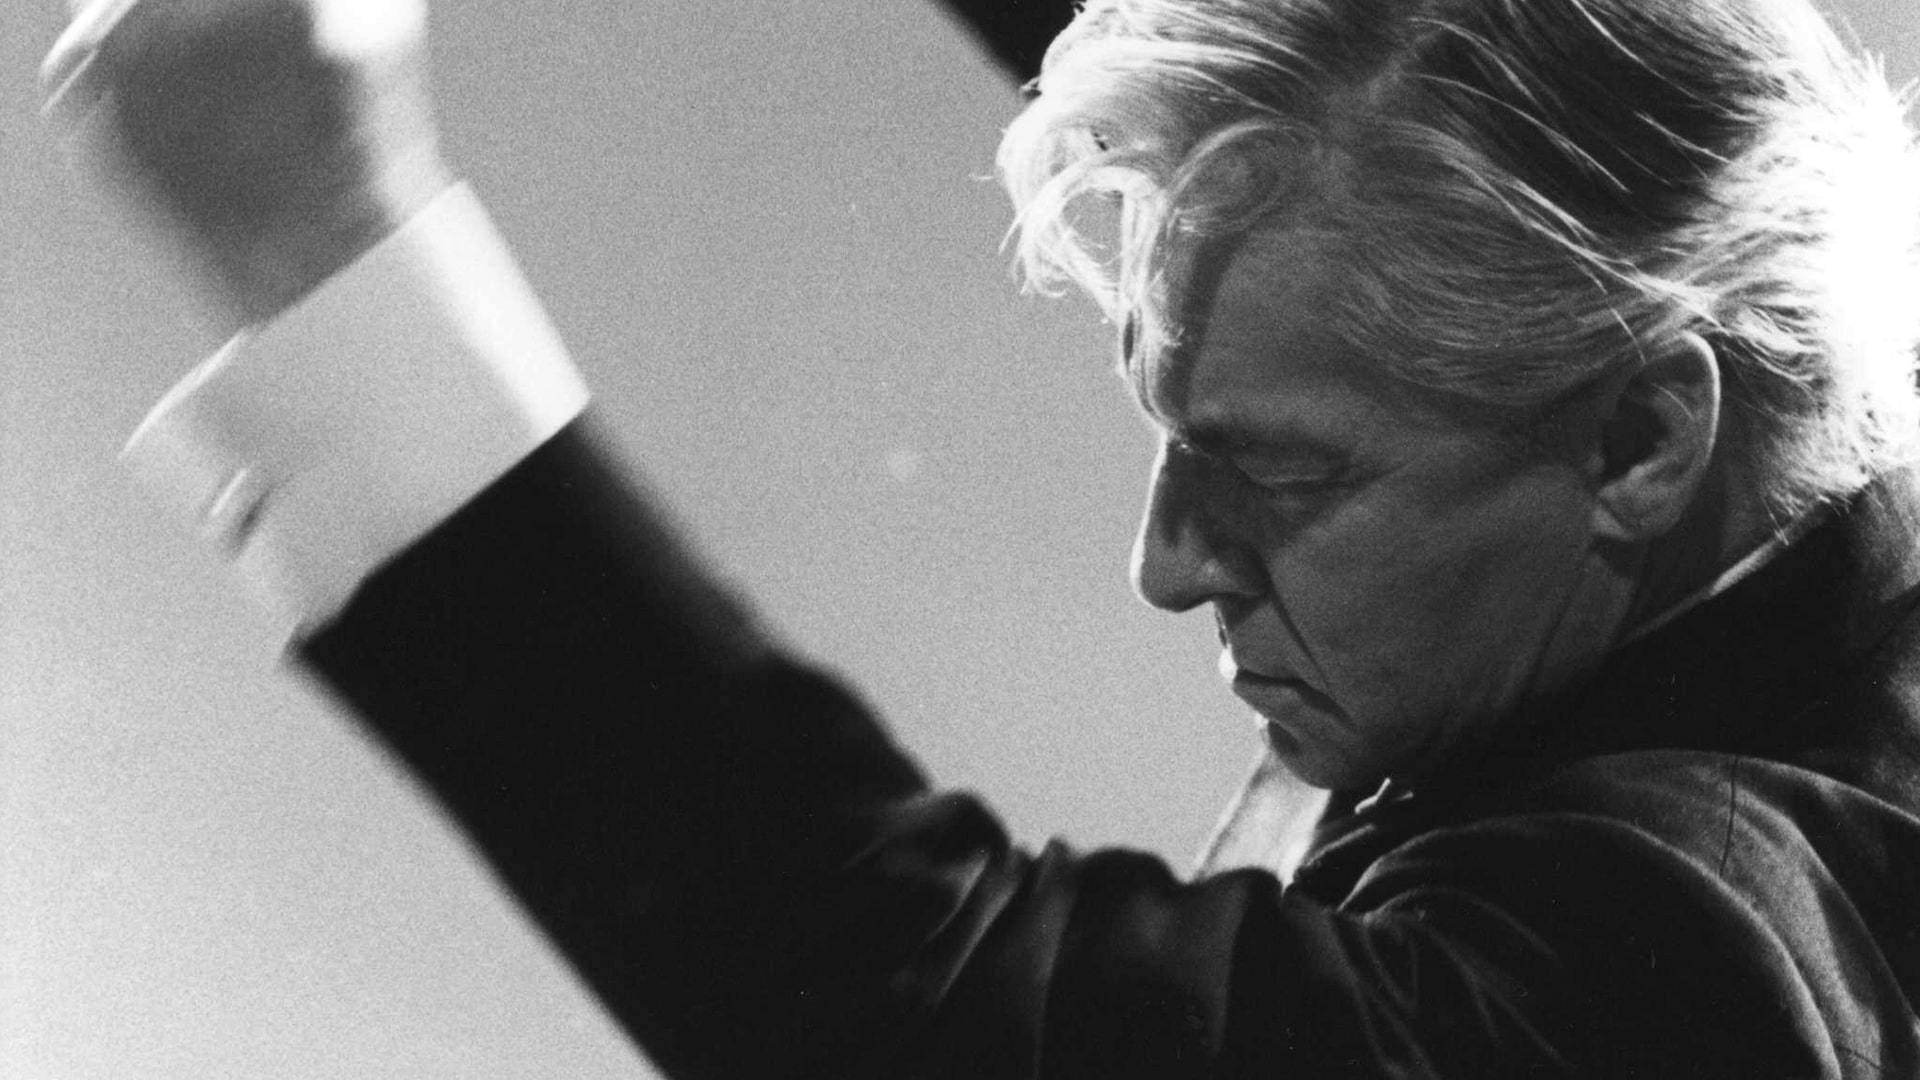
\includegraphics[width = .5\textwidth]{resources/Herbert_von_Karajan.jpg}
    \label{fig:hvk}
\end{figure}
\begin{figure}[H]
\centering
    \begin{minipage}{.5\textwidth}
    \centering
    \caption{Восстановленное изображение \\(50 компонент)}
    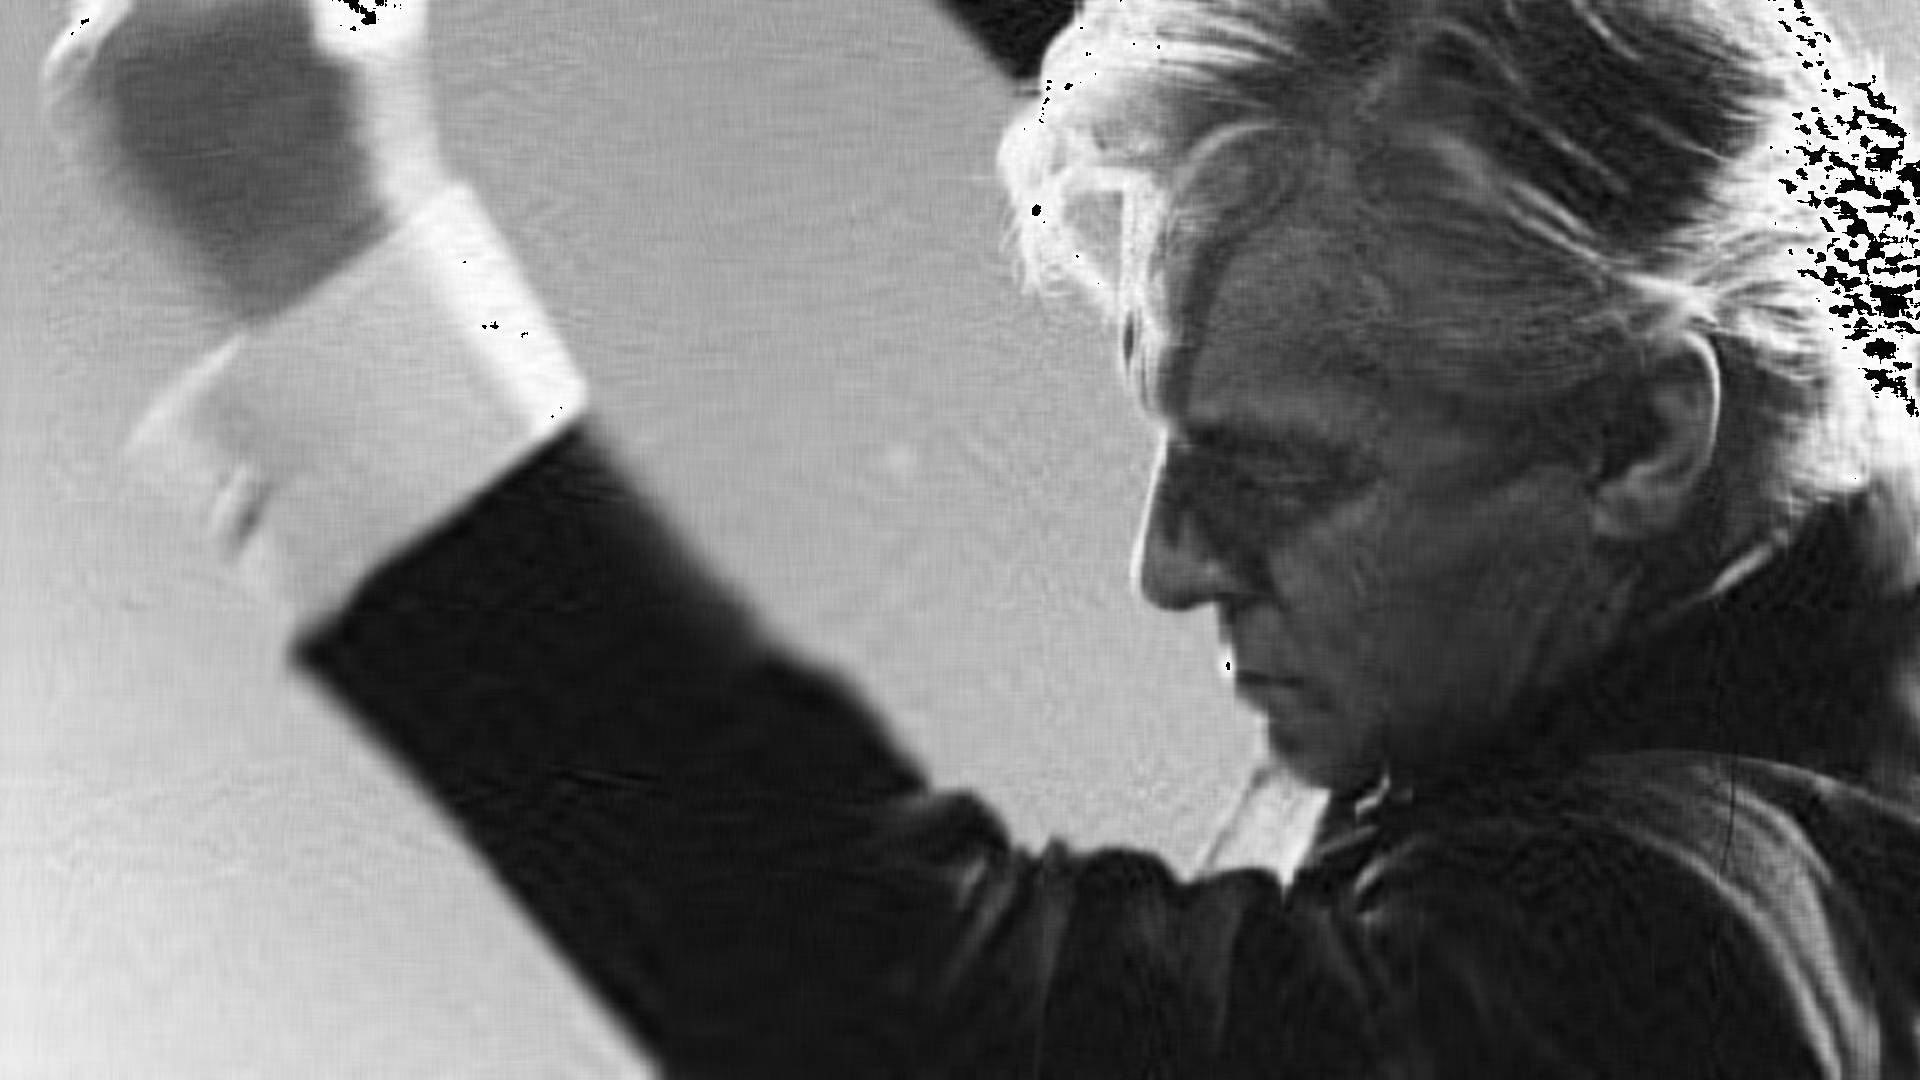
\includegraphics[width = 0.95\textwidth]{reconstructions/with_50comps_Herbert_von_Karajan.jpg}
    \label{fig:hvk_50}
    \end{minipage}%
    \begin{minipage}{.5\textwidth}
    \caption{Восстановленное изображение \\(100 компонент)}
    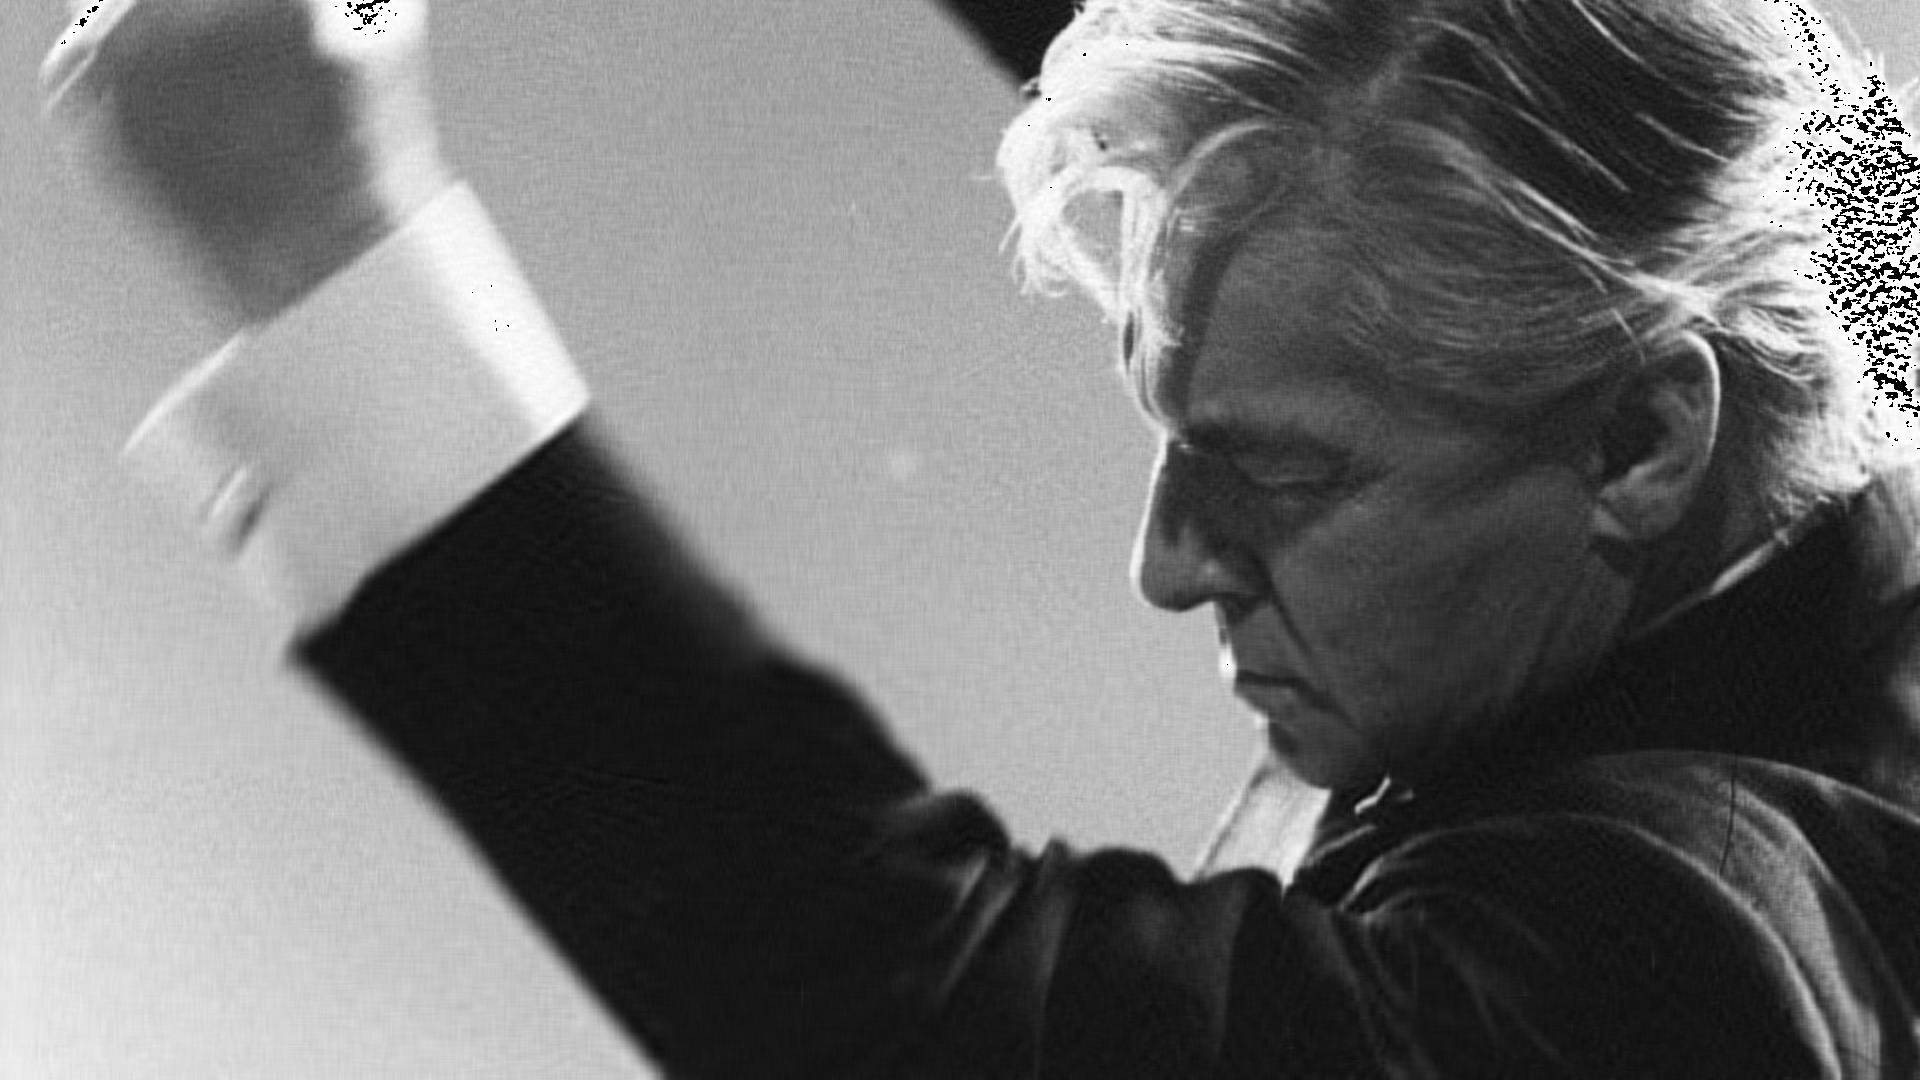
\includegraphics[width = 0.95\textwidth]{reconstructions/with_100comps_Herbert_von_Karajan.jpg}
    \label{fig:hvk_100}
    \end{minipage}%
\end{figure}
\begin{figure}[H]
    \centering
    \caption{Восстановленное изображение \\(200 компонент)}
    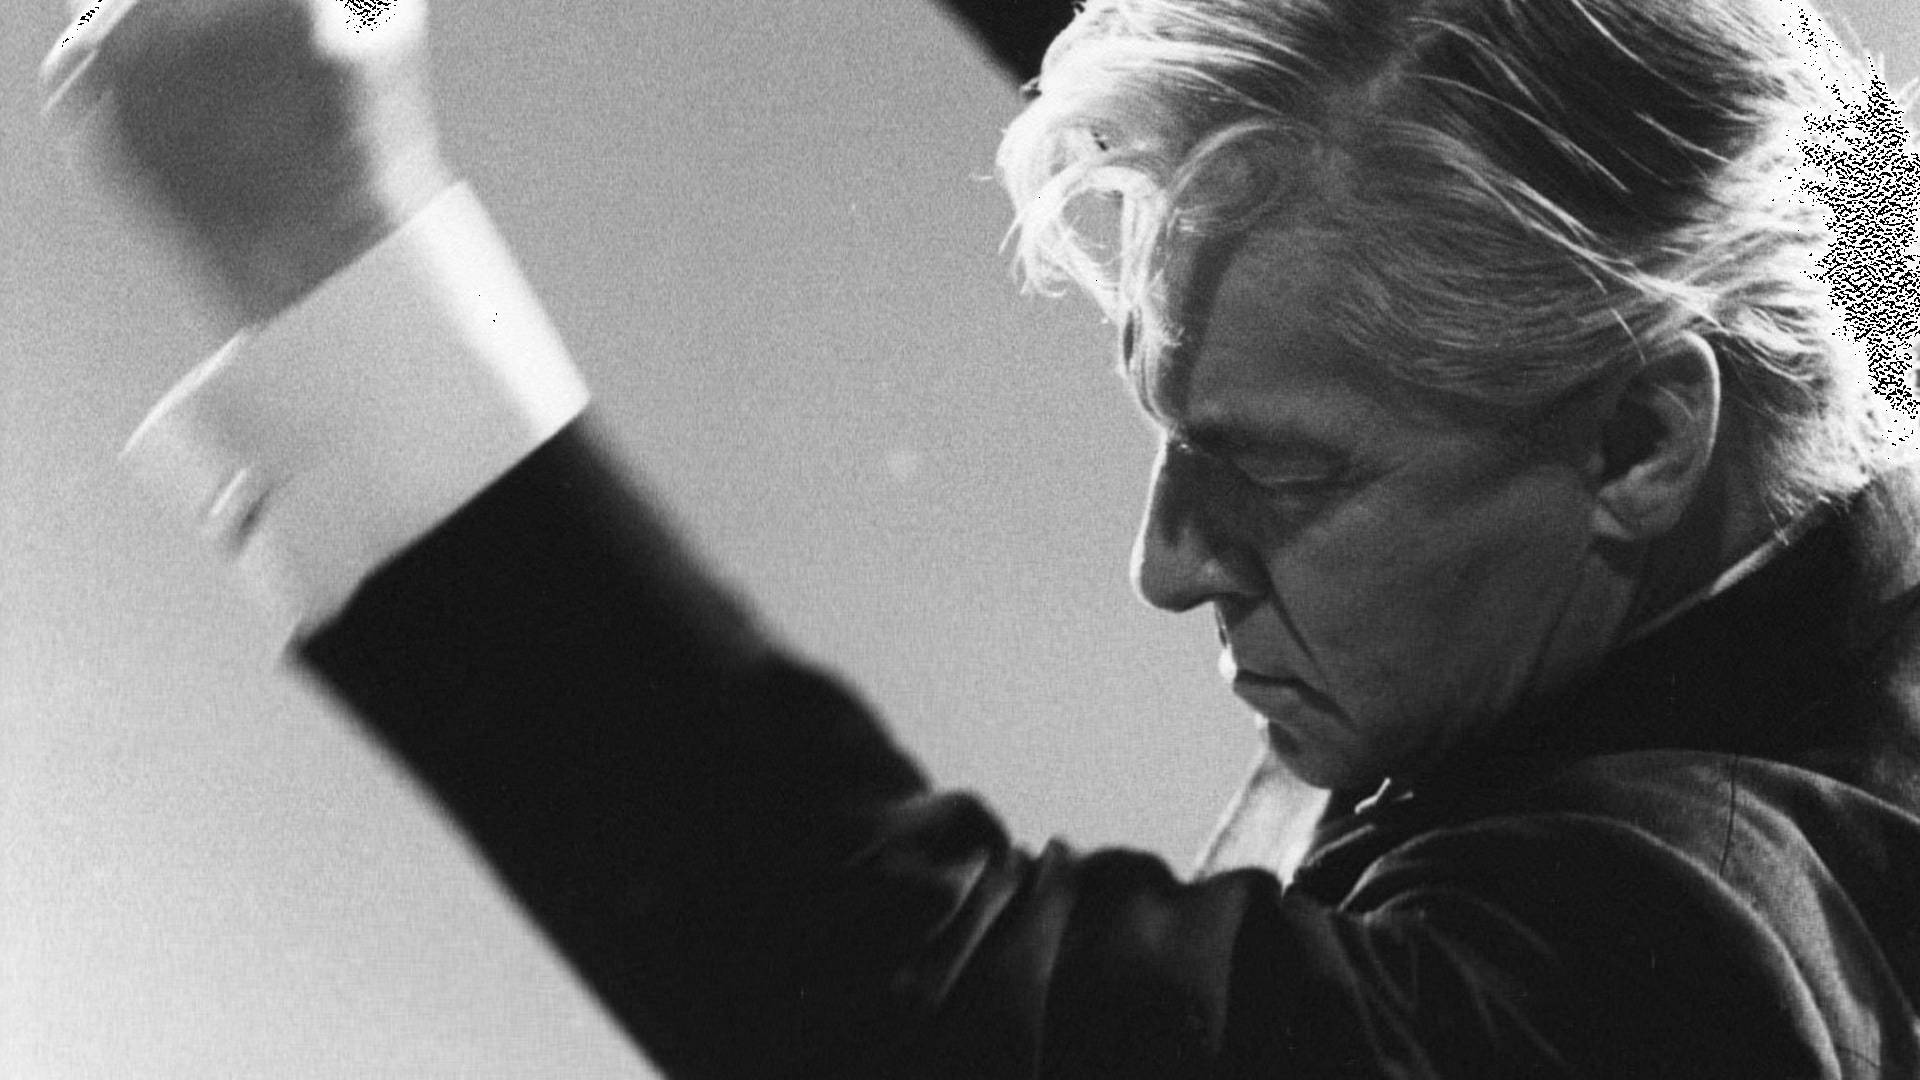
\includegraphics[width = .5\textwidth]{reconstructions/with_200comps_Herbert_von_Karajan.jpg}
    \label{fig:hvk_200}
\end{figure}
\begin{table}[H]
    \centering
    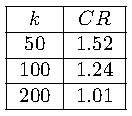
\includegraphics[]{tables/CR_for_Herbert_von_Karajan.pdf}
    \caption{Оценка сжатия первого\\черно-белого рисунка}
    \label{tab:hvk}
\end{table}
\newpage
\subsubsection{Второе изображение}
Размер оригинала - 1.77 МБ, разрешение - $3000\times 2402$ пикселя.
\begin{figure}[H]
\centering
\caption{Оригинал}
    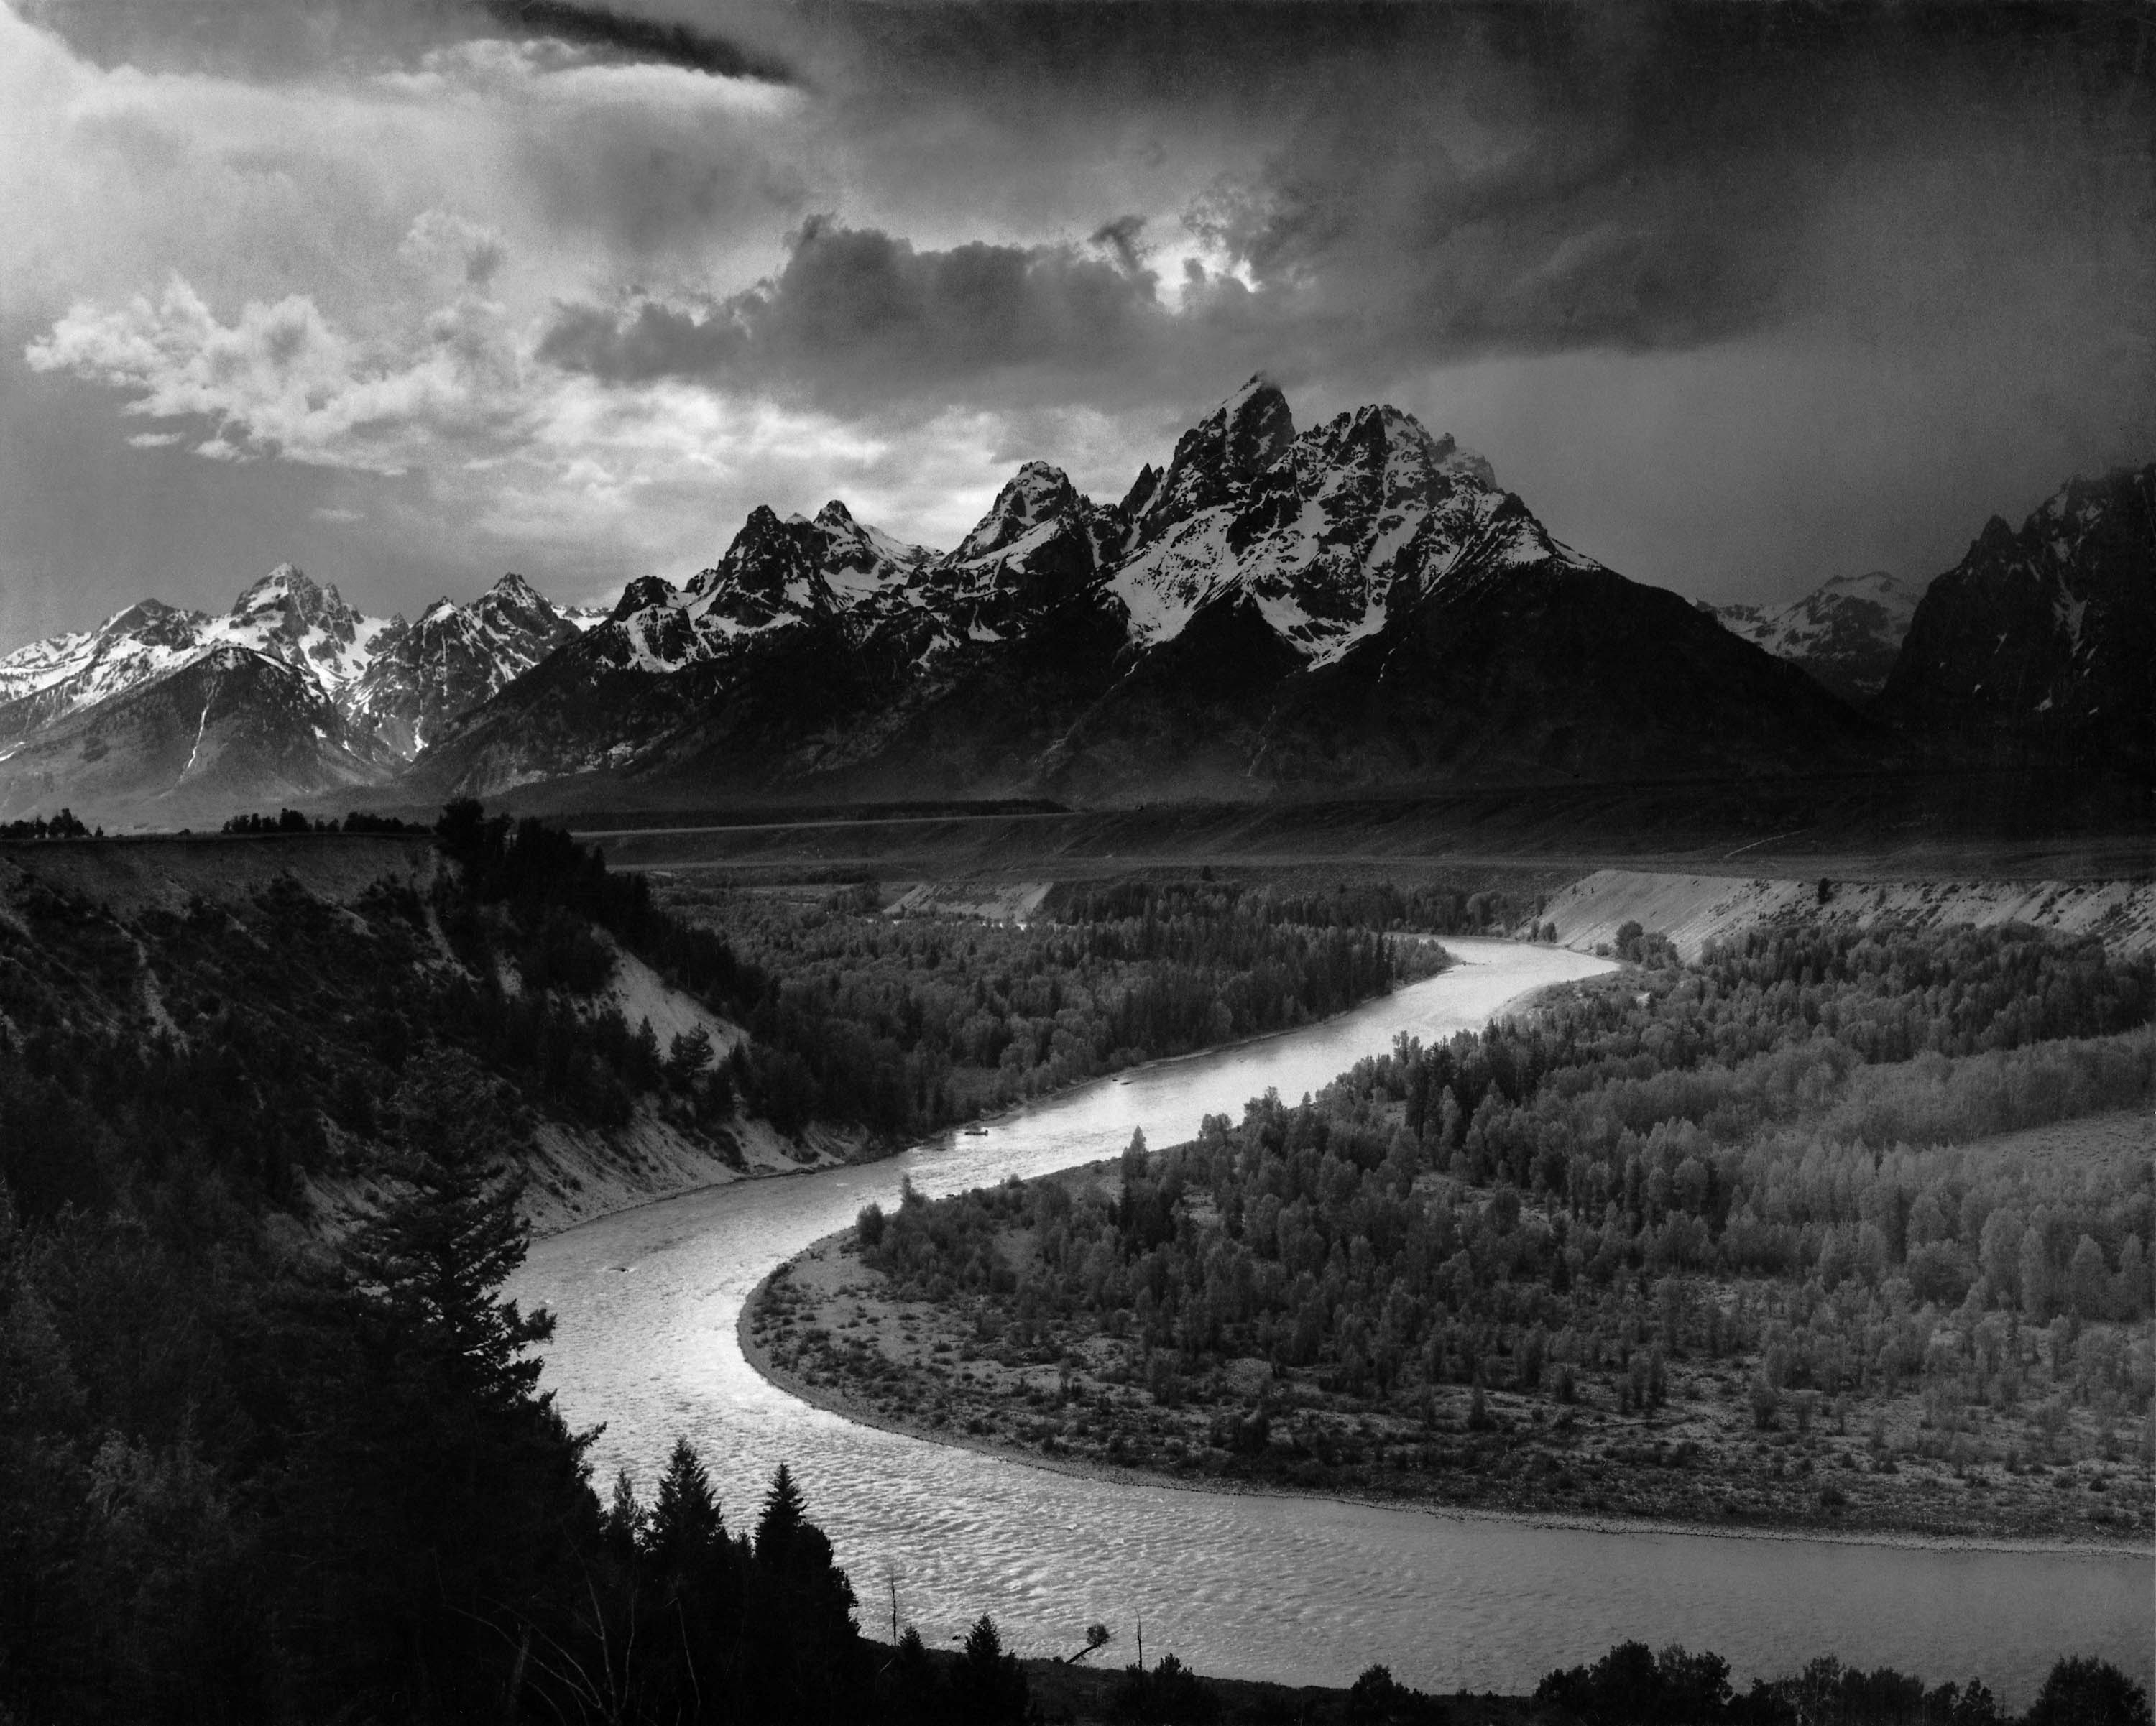
\includegraphics[width = 0.5\textwidth]{resources/Adams_The_Tetons_and_the_Snake_River.jpg}
    \label{fig:mount_orig}
\end{figure}
\begin{figure}[H]
\centering
    \begin{minipage}{.5\textwidth}
    \caption{Восстановленное изображение \\(50 компонент)}
    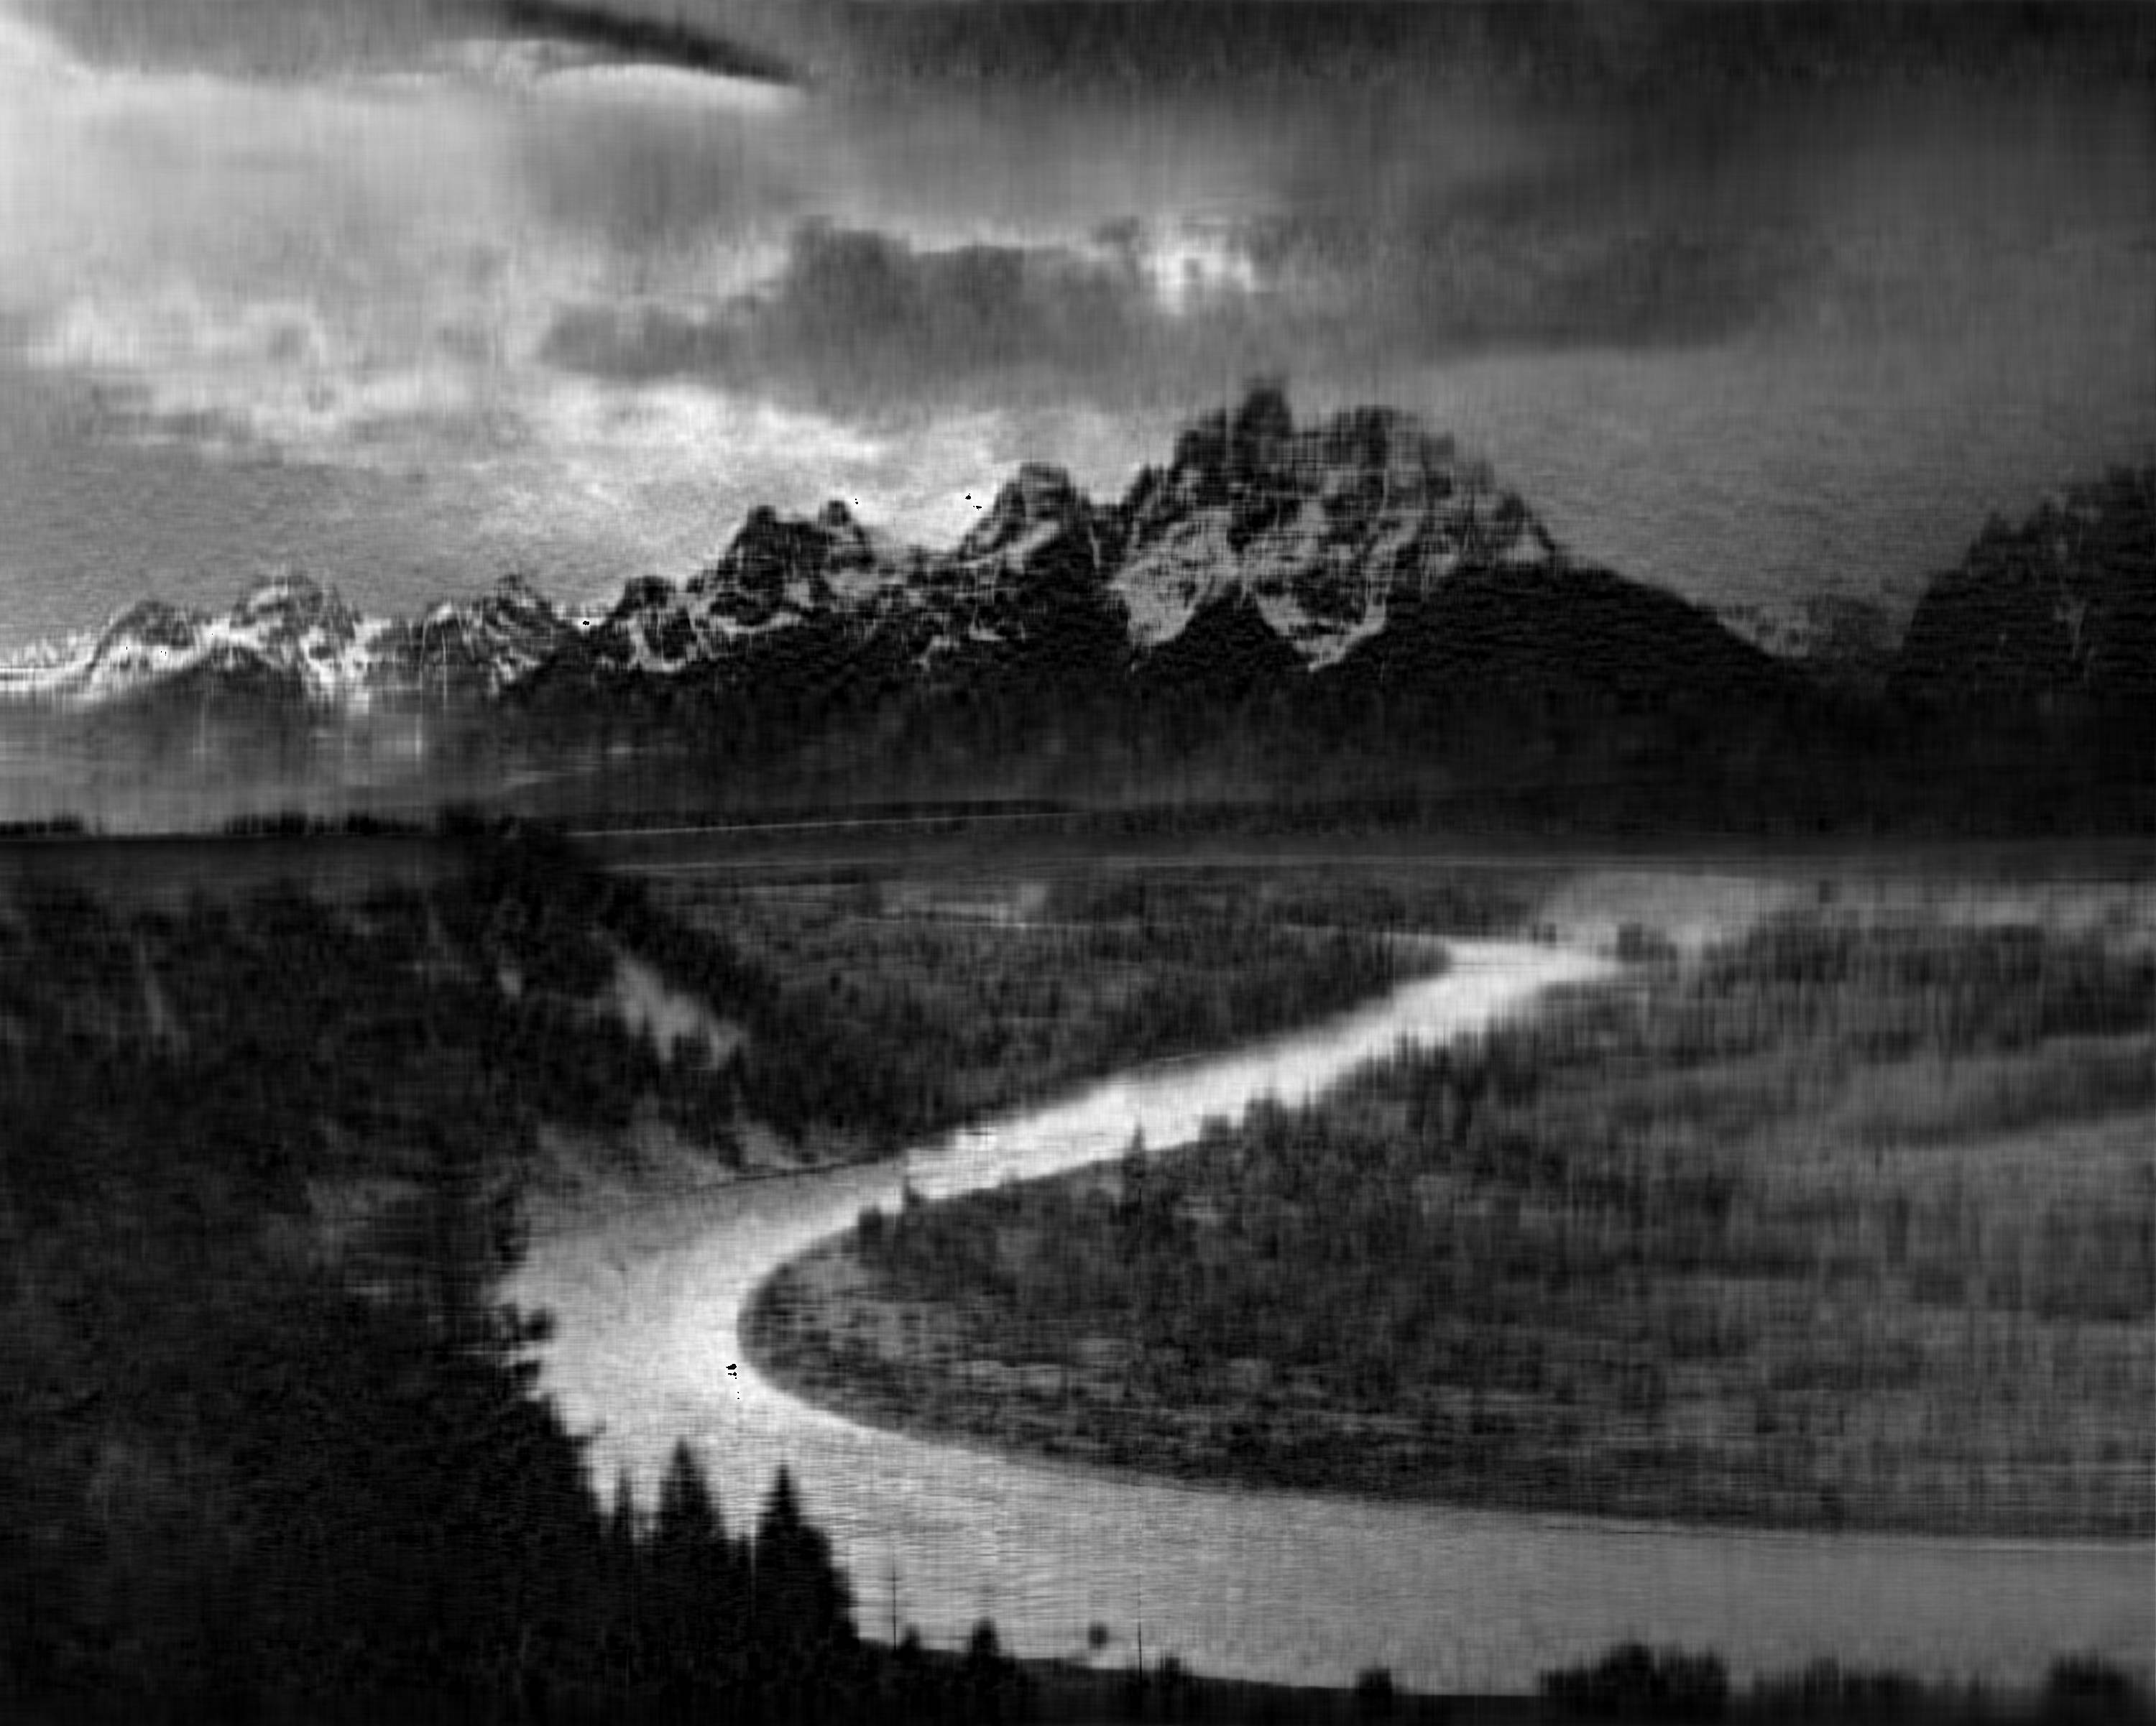
\includegraphics[width = 0.95\textwidth]{reconstructions/with_50comps_Adams_The_Tetons_and_the_Snake_River.jpg}
    \label{fig:mount_50}
    \hspace{8 mm}
    \caption{Восстановленное изображение \\(200 компонент)}
    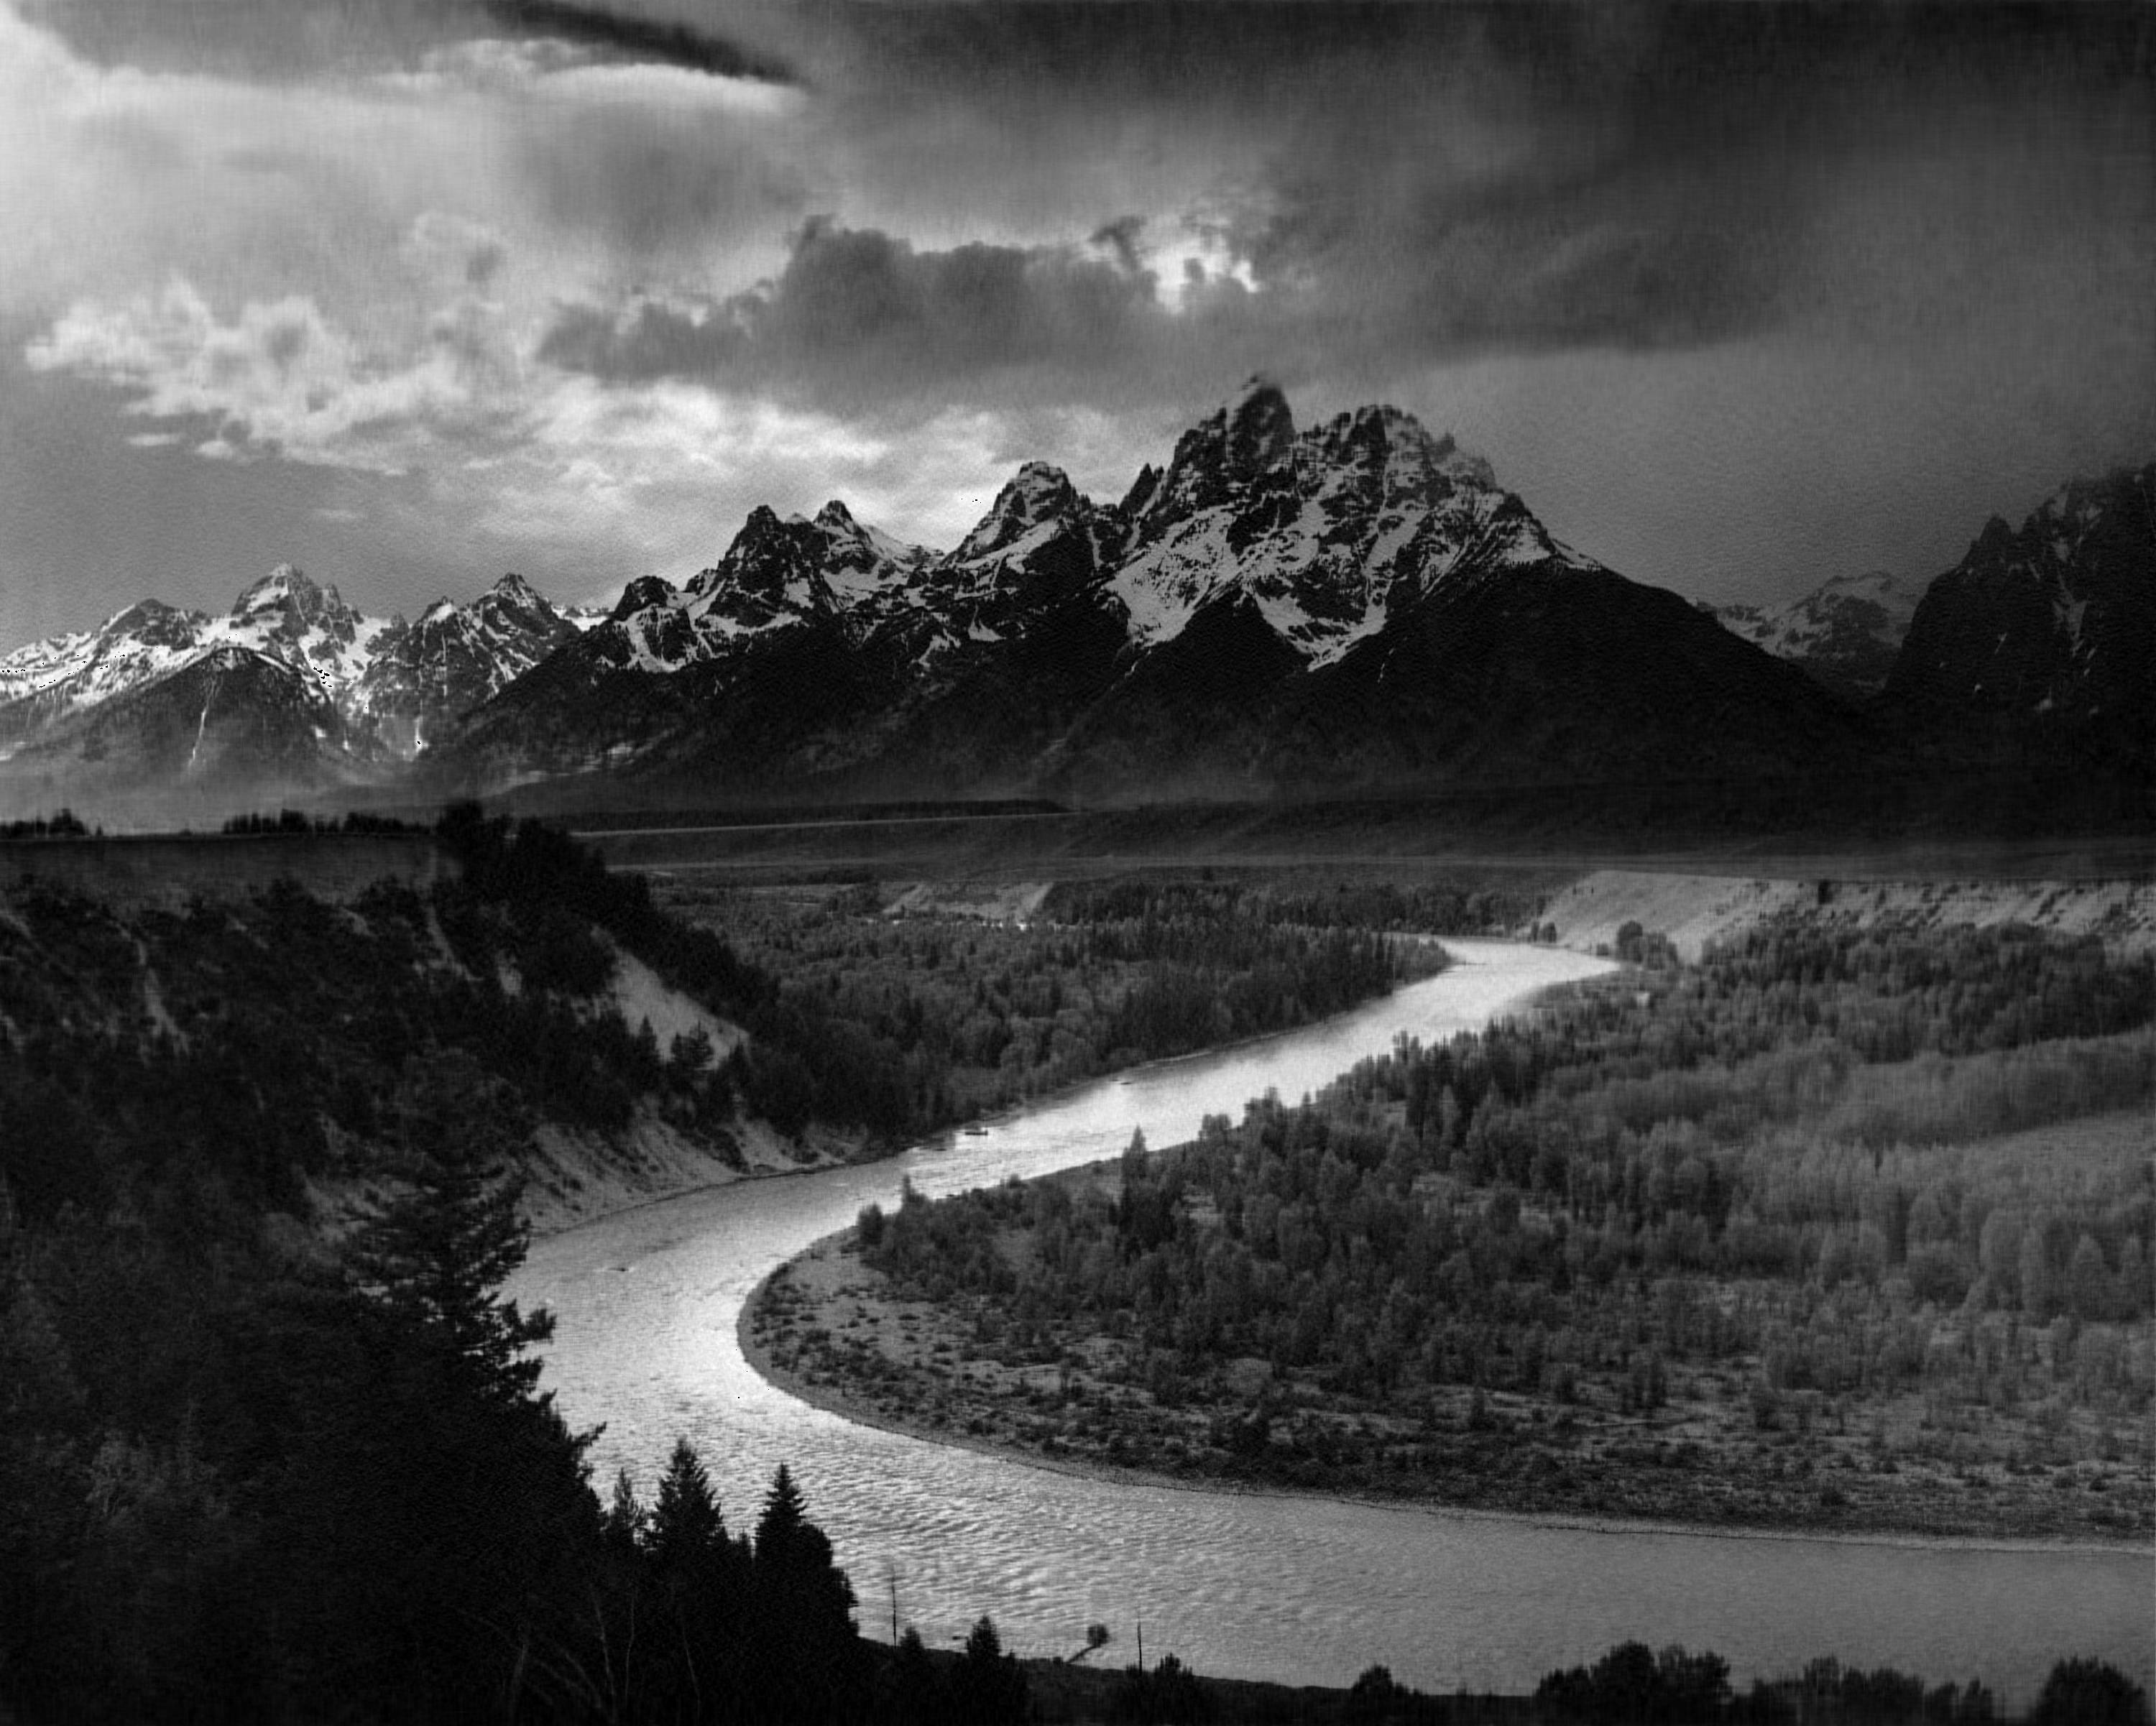
\includegraphics[width = 0.95\textwidth]{reconstructions/with_200comps_Adams_The_Tetons_and_the_Snake_River.jpg}
    \label{fig:mount_200}
    \end{minipage}%
    \begin{minipage}{.5\textwidth}
      \centering
    \caption{Восстановленное изображение \\(100 компонент)}
    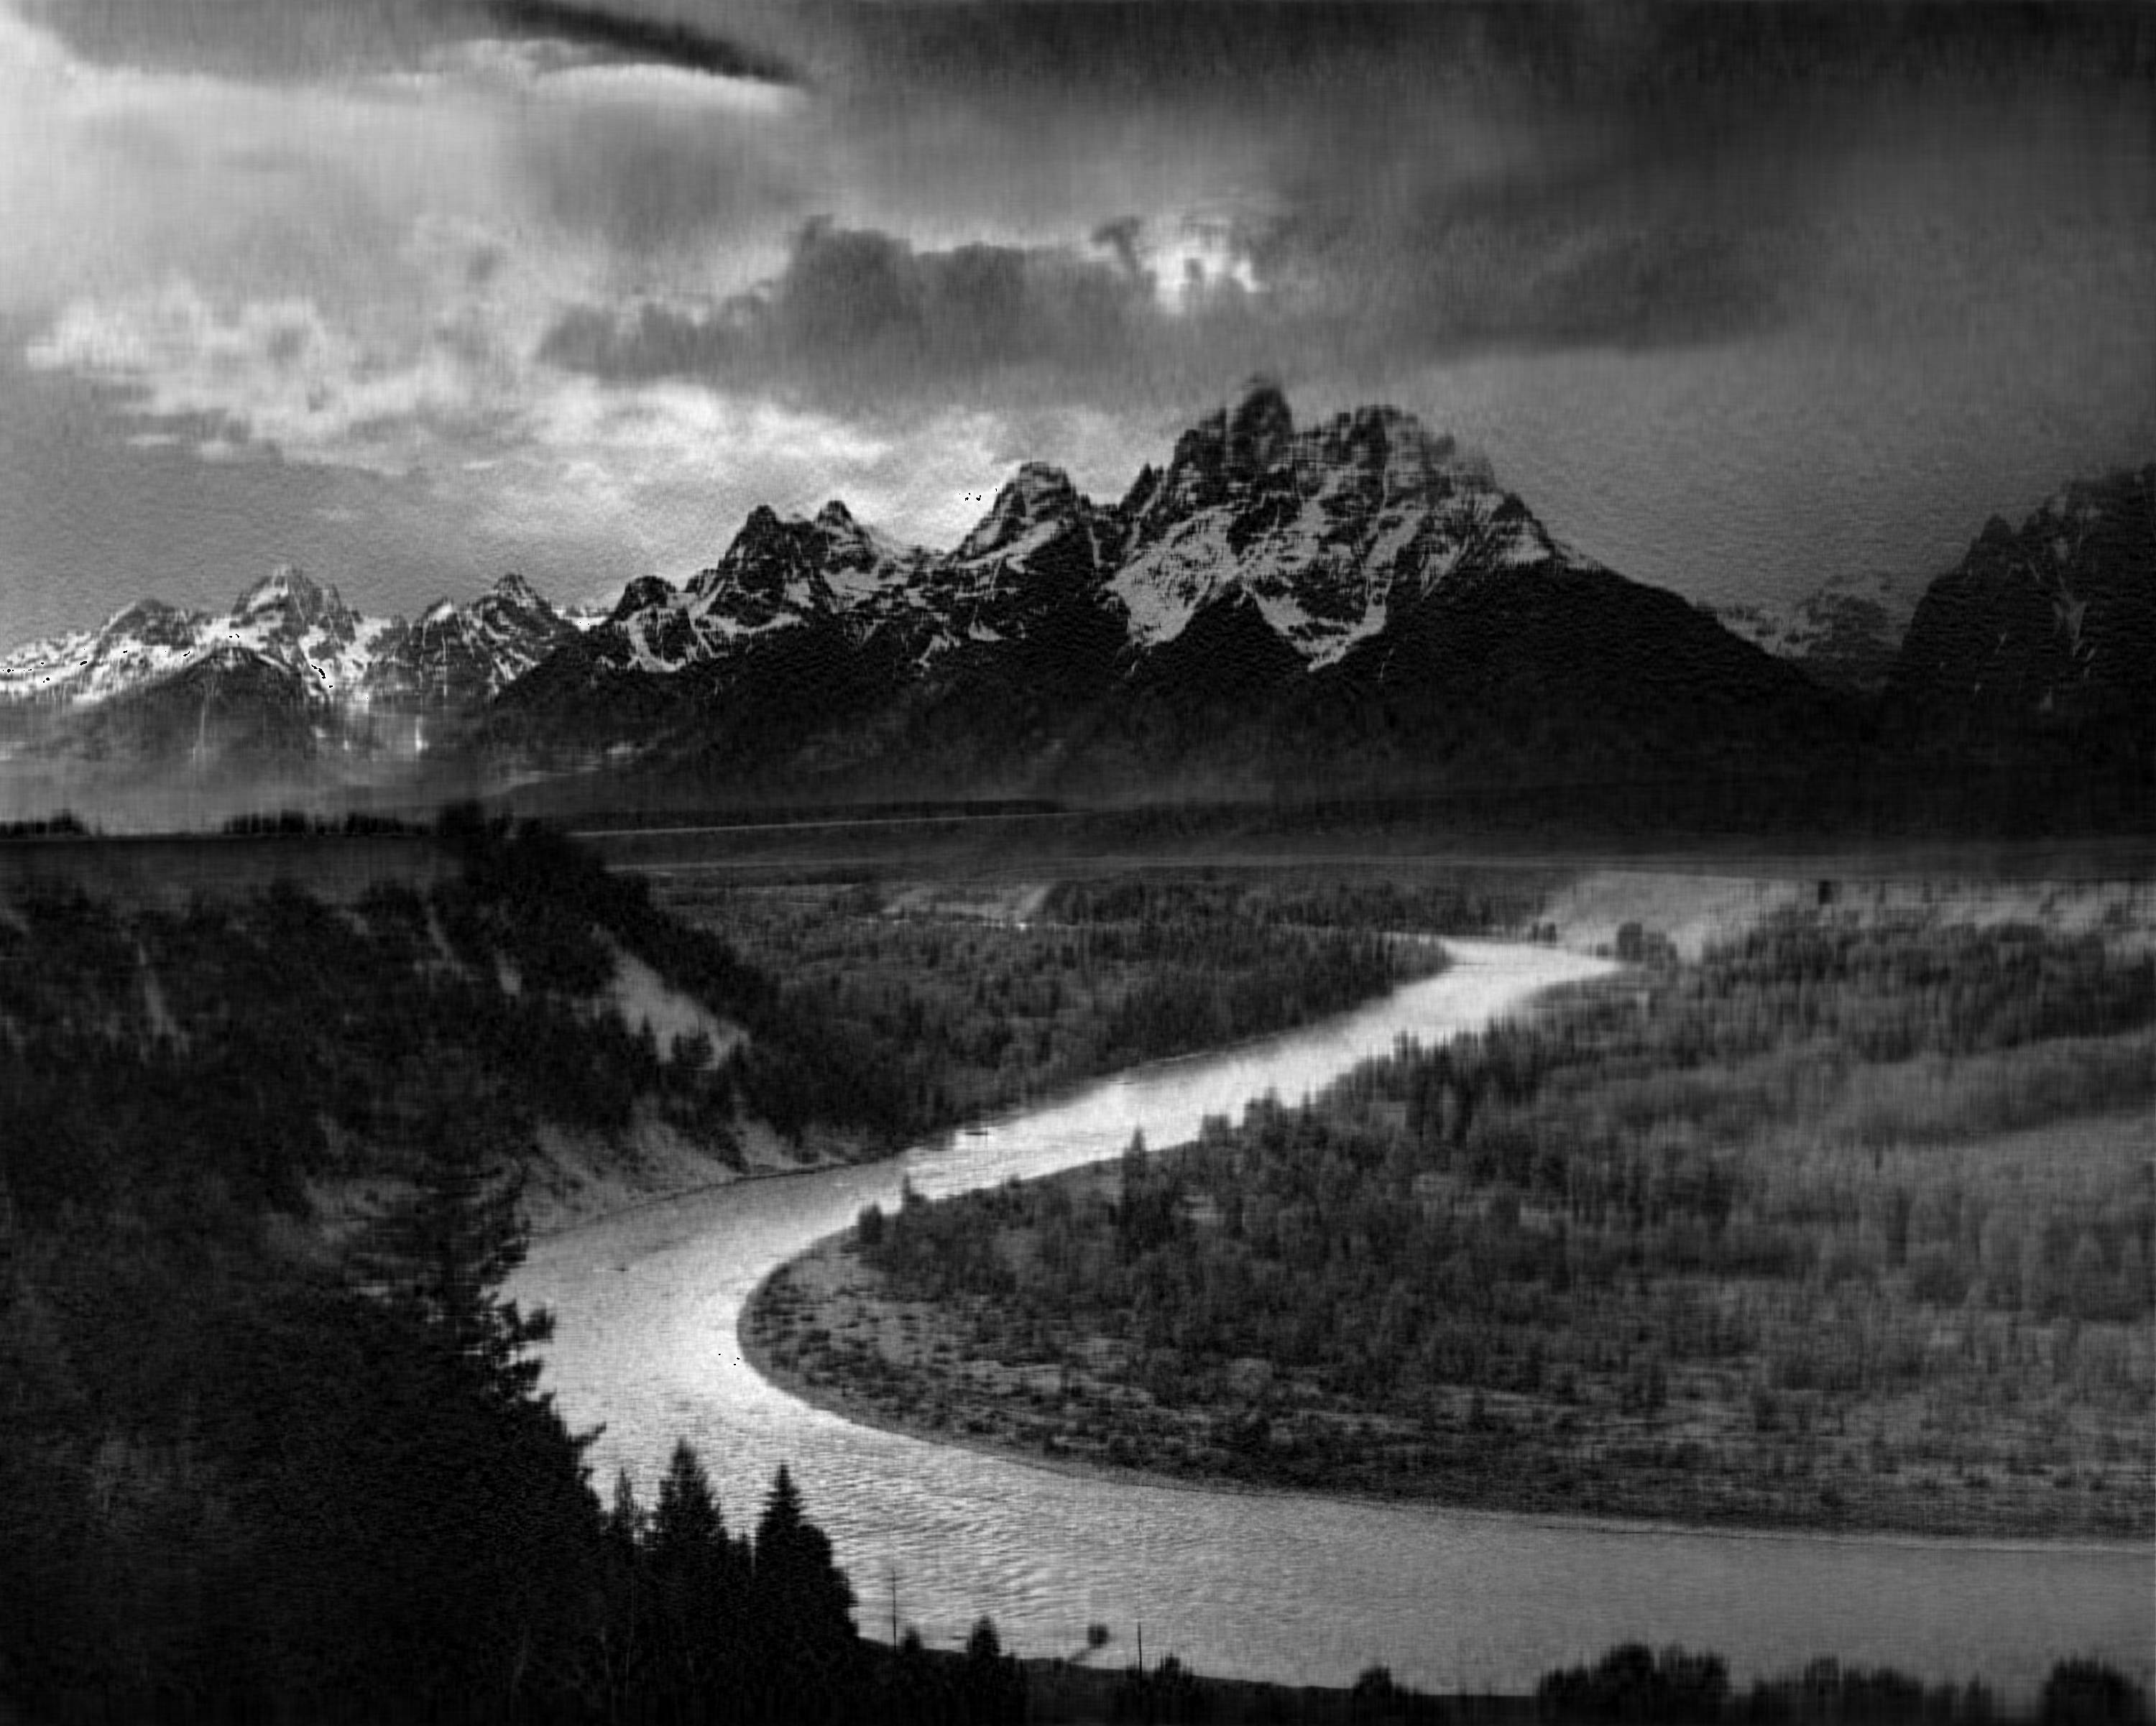
\includegraphics[width = 0.95\textwidth]{reconstructions/with_100comps_Adams_The_Tetons_and_the_Snake_River.jpg}
    \label{fig:mount_100}
    \hspace{8 mm}
    \caption{Восстановленное изображение \\(400 компонент)}
    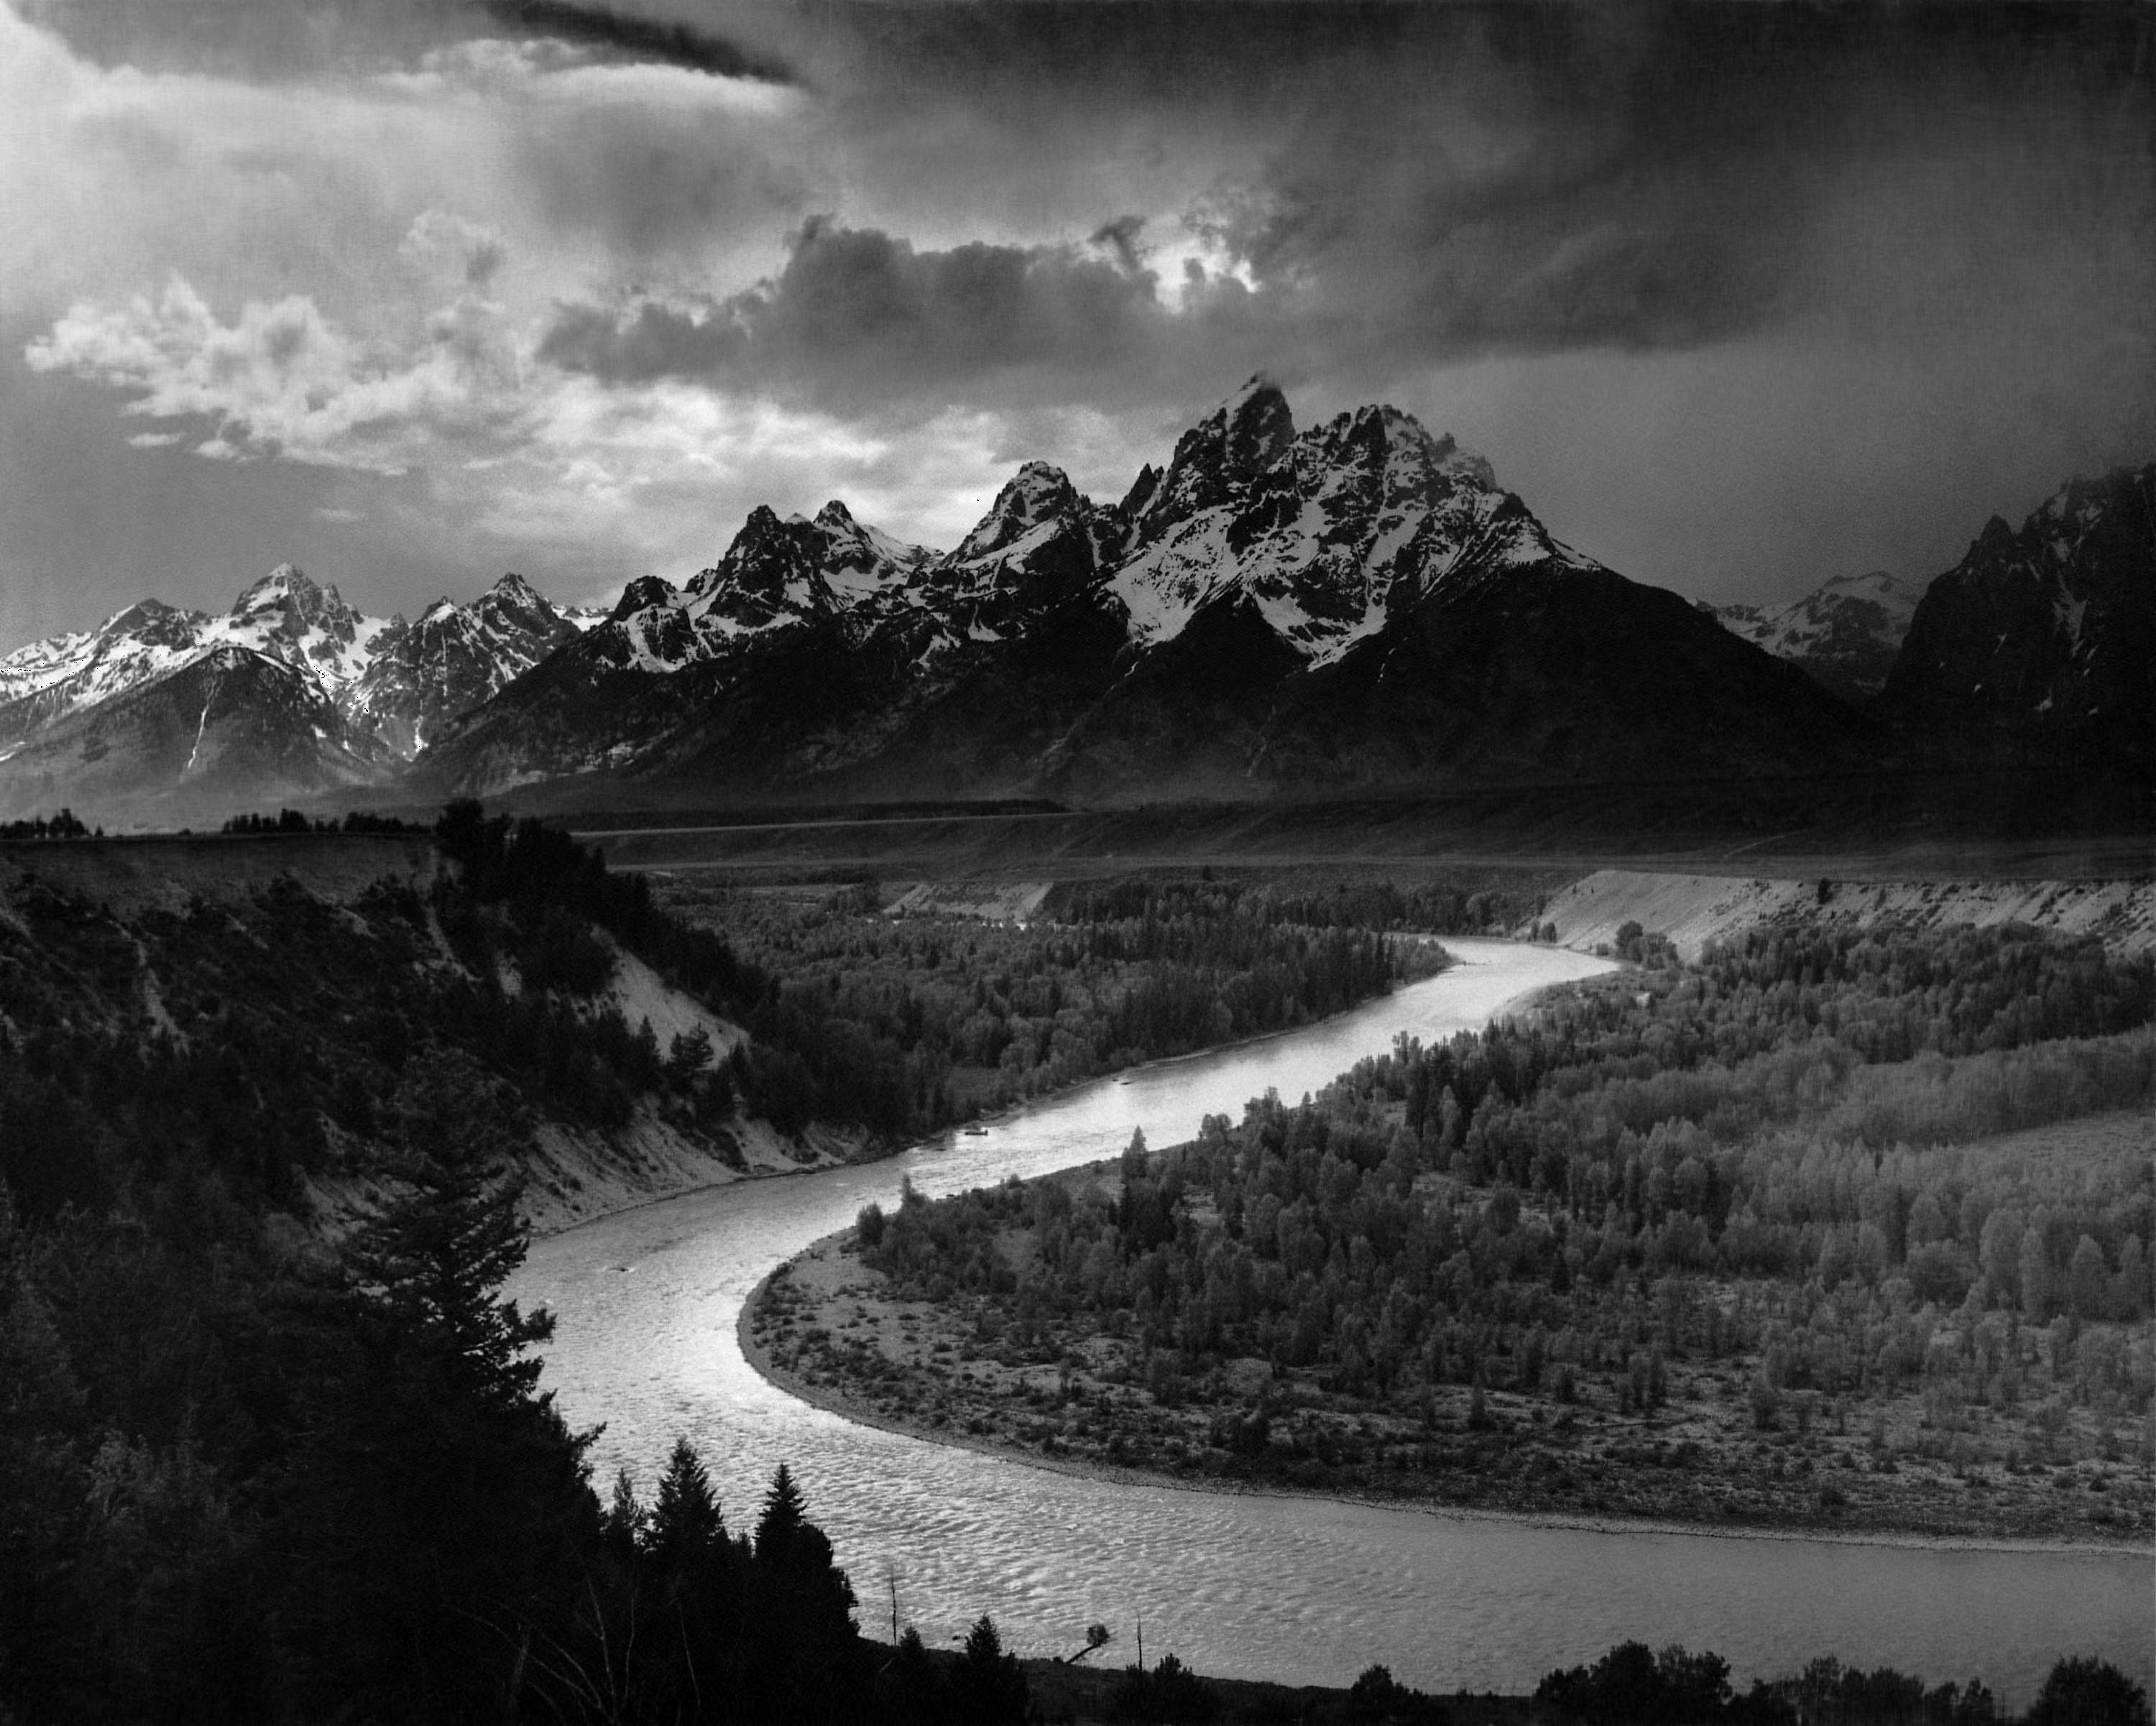
\includegraphics[width = 0.95\textwidth]{reconstructions/with_400comps_Adams_The_Tetons_and_the_Snake_River.jpg}
    \label{fig:mount_400}
    \end{minipage}%
\end{figure}
\begin{table}[H]
    \centering
    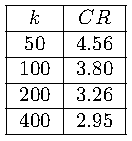
\includegraphics[]{tables/CR_for_Adams_The_Tetons_and_the_Snake_River.pdf}
    \caption{Оценка сжатия второго\\черно-белого рисунка}
    \label{tab:mount}
\end{table}
\subsection{Цветные изображения}
\subsubsection{Первое изображение}
Размер оригинала - 483 КБ, разрешение - $1920\times 1080$ пикселя.
\begin{figure}[H]
\centering
\caption{Оригинал}
    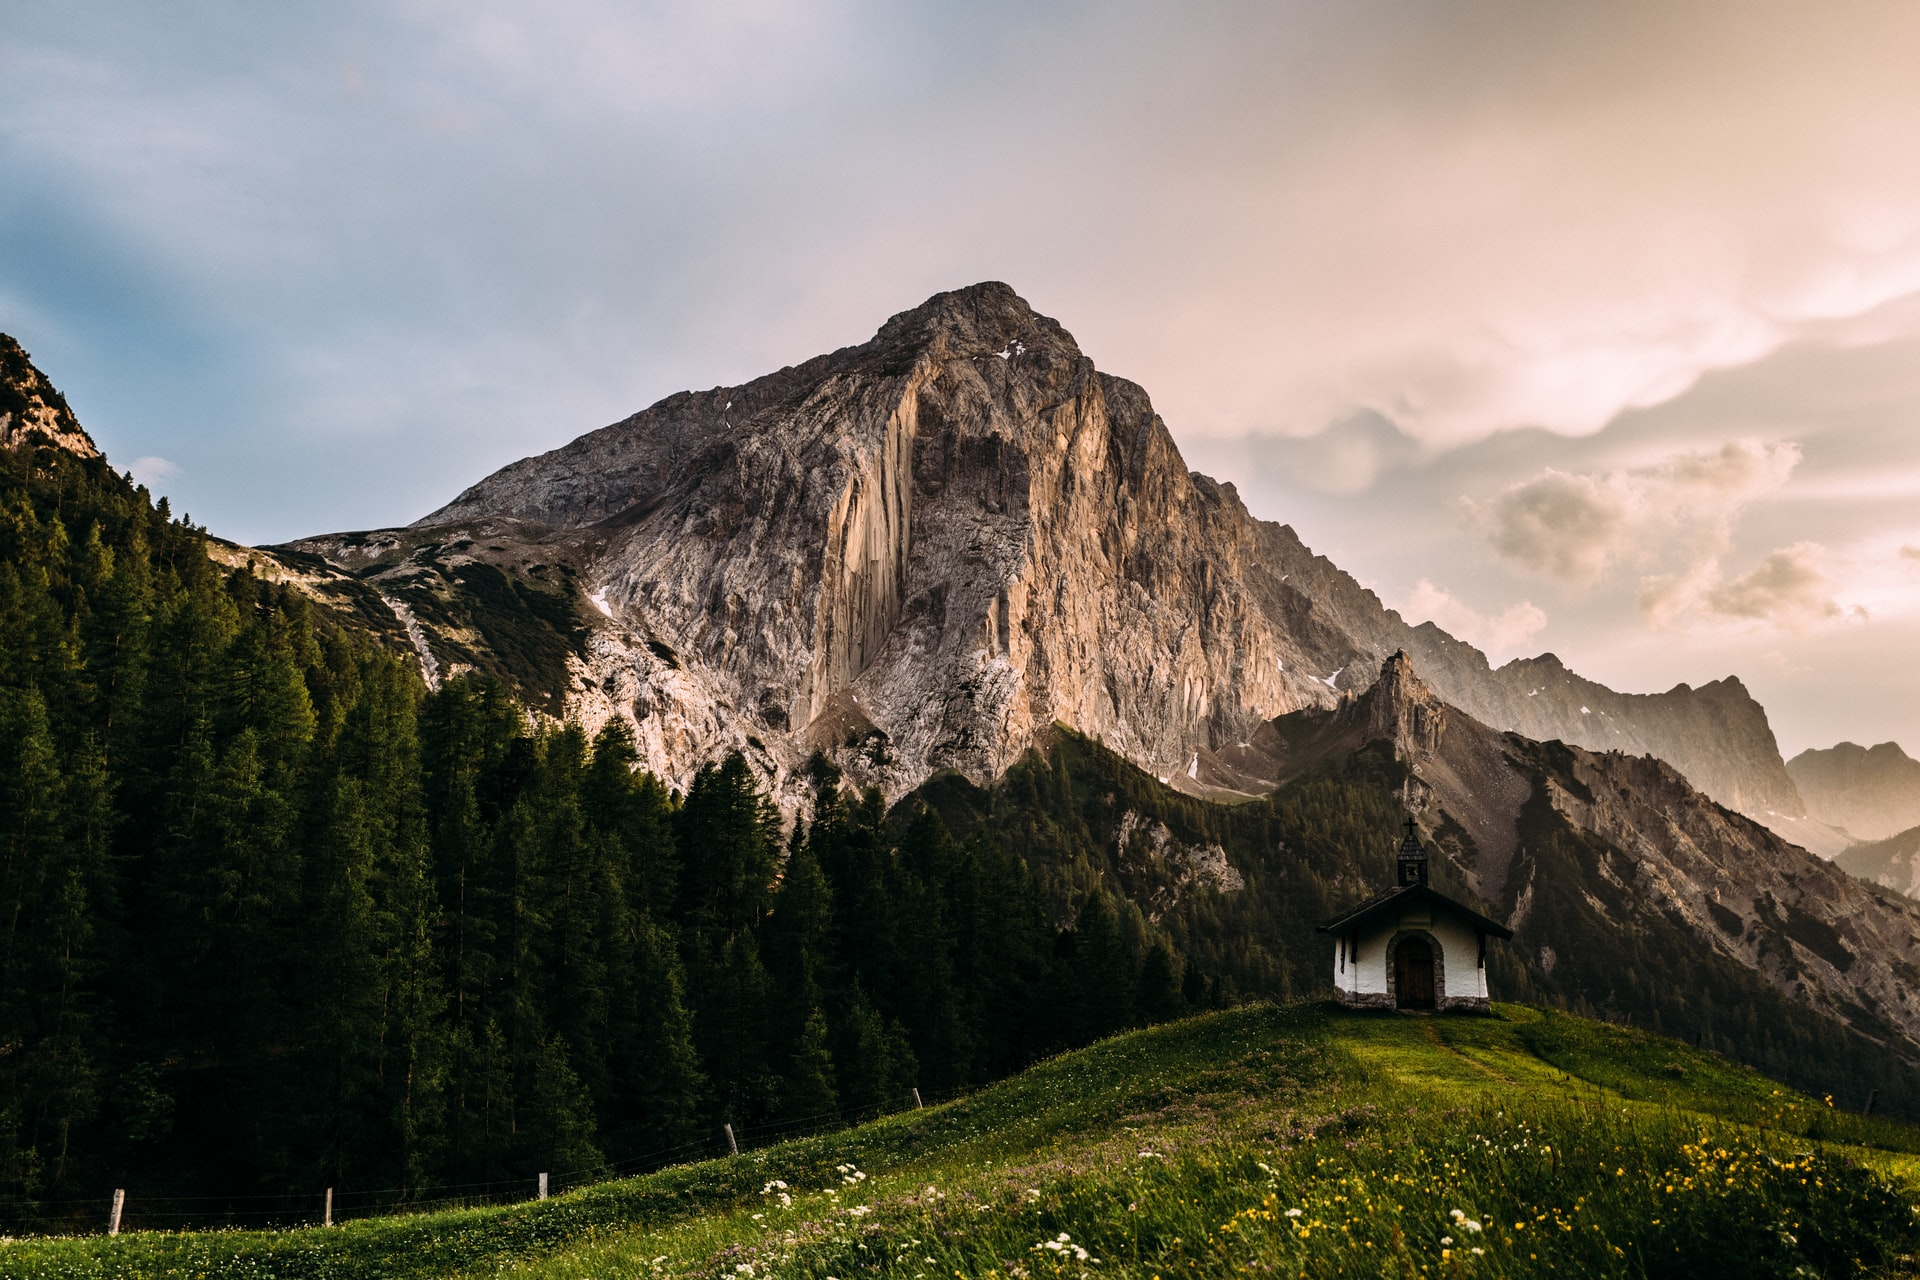
\includegraphics[width = 0.45\textwidth]{resources/Austria.jpg}
    \label{fig:aus_orig}
\end{figure}
\begin{figure}[H]
\centering
    \begin{minipage}{.45\textwidth}
    \caption{Восстановленное изображение \\(50 компонент)}
    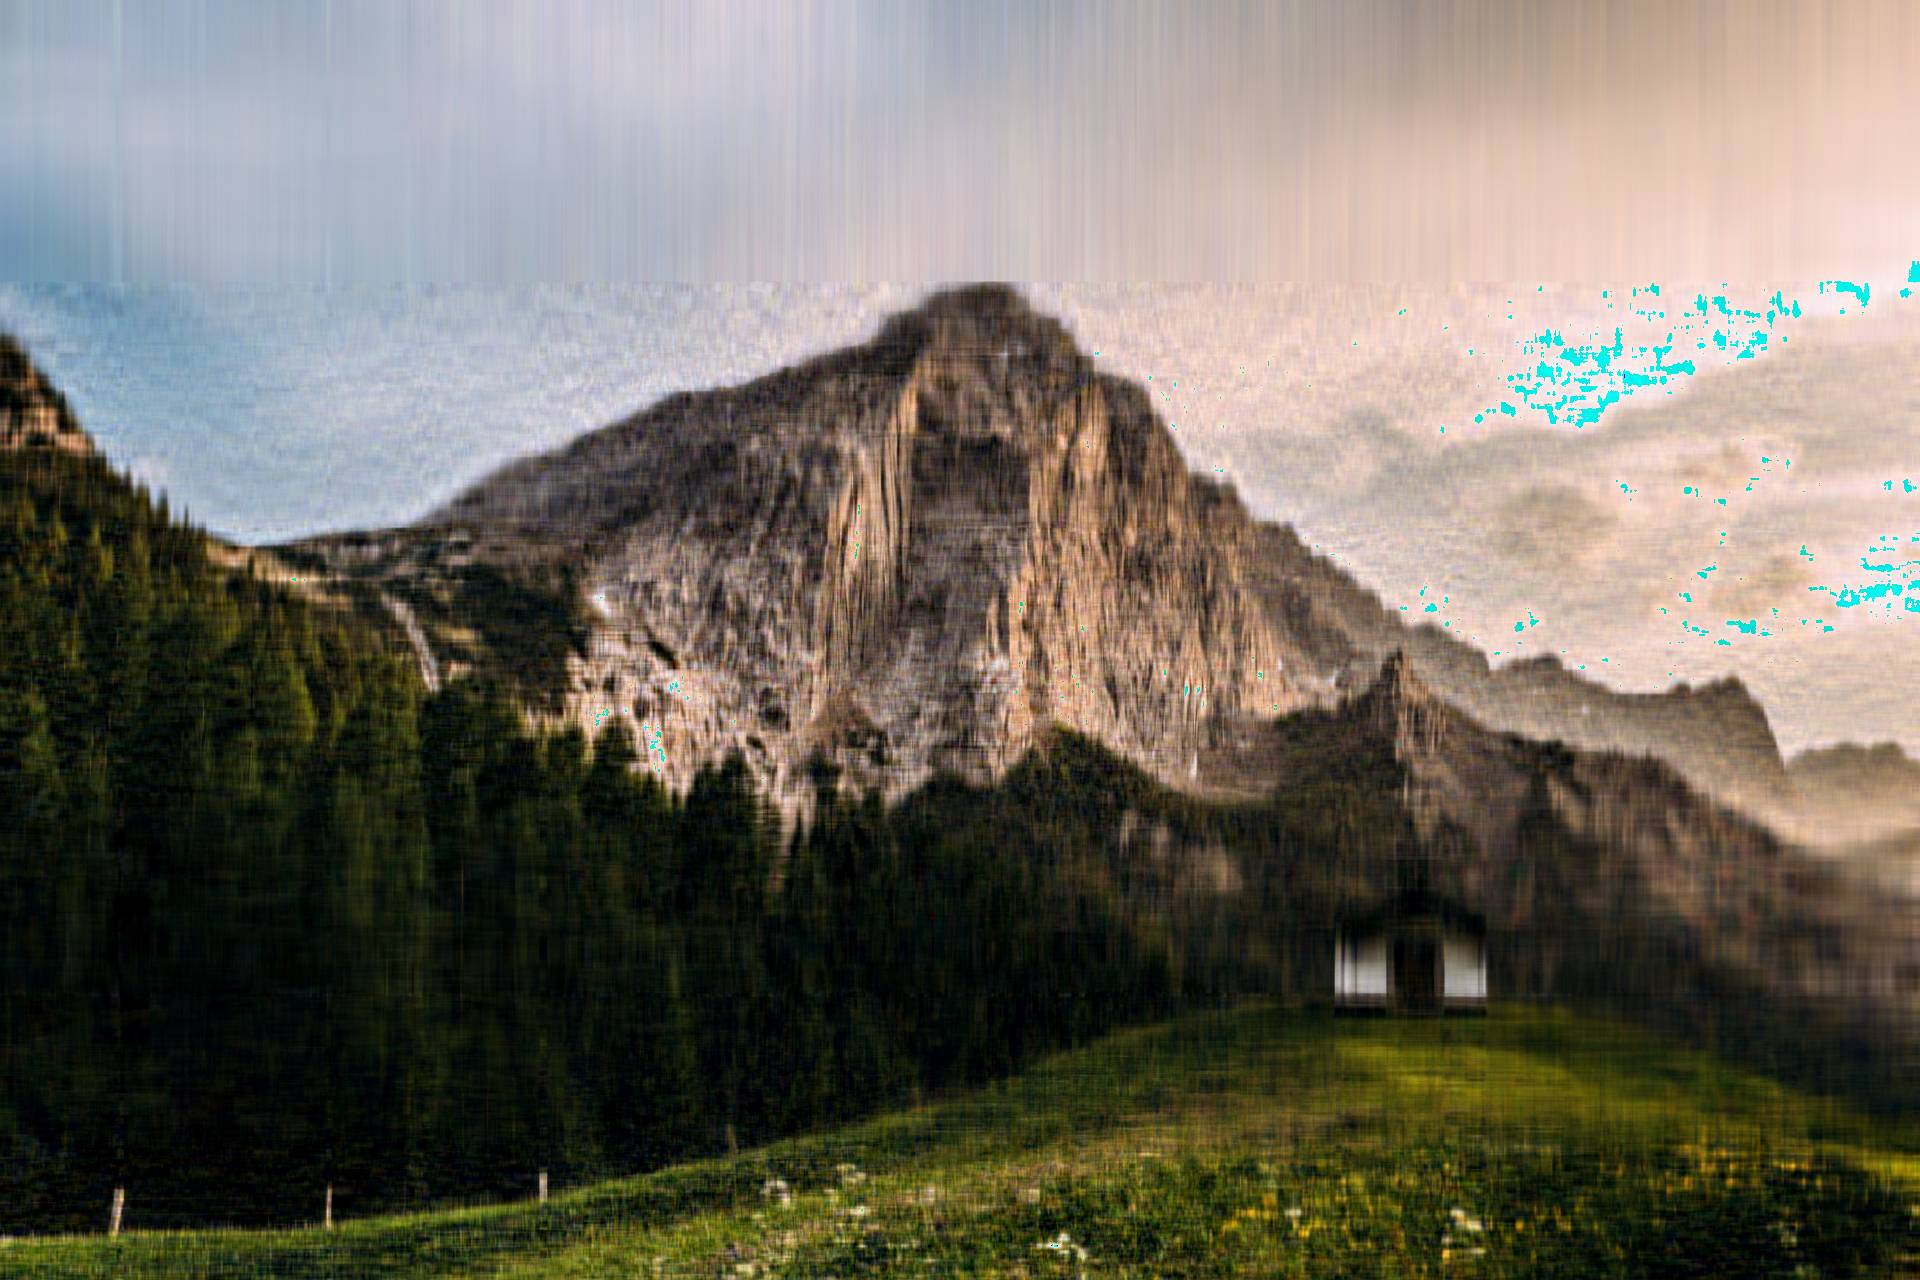
\includegraphics[width = 0.95\textwidth]{reconstructions/with_50comps_Austria.jpg}
    \label{fig:aus_50}
    \end{minipage}%
    \begin{minipage}{.45\textwidth}
      \centering
    \caption{Восстановленное изображение \\(100 компонент)}
    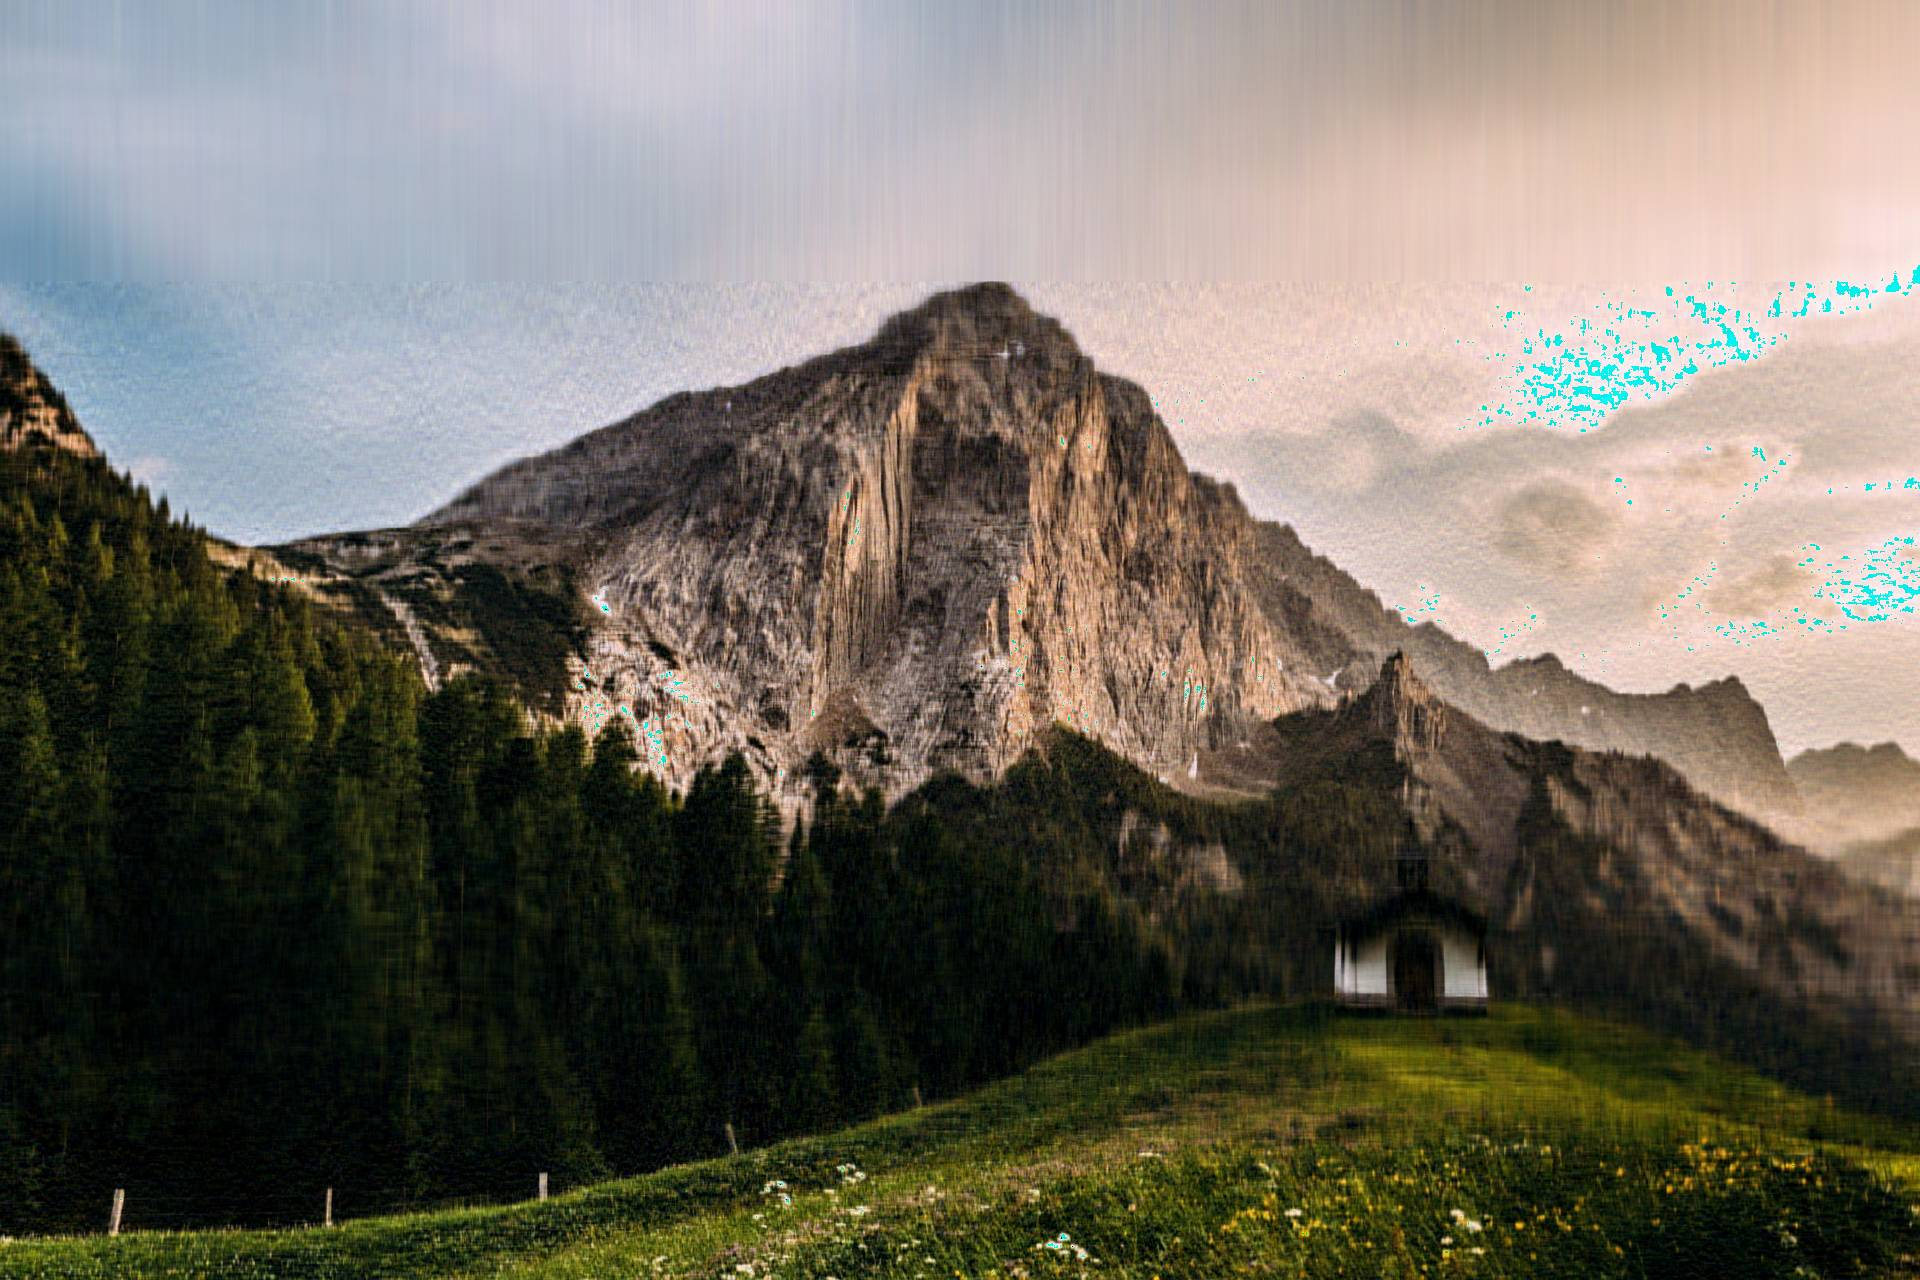
\includegraphics[width = 0.95\textwidth]{reconstructions/with_100comps_Austria.jpg}
    \label{fig:aus_100}
    \end{minipage}%
\end{figure}
\begin{figure}[H]
\centering
    \begin{minipage}{.45\textwidth}
    \caption{Восстановленное изображение \\(200 компонент)}
    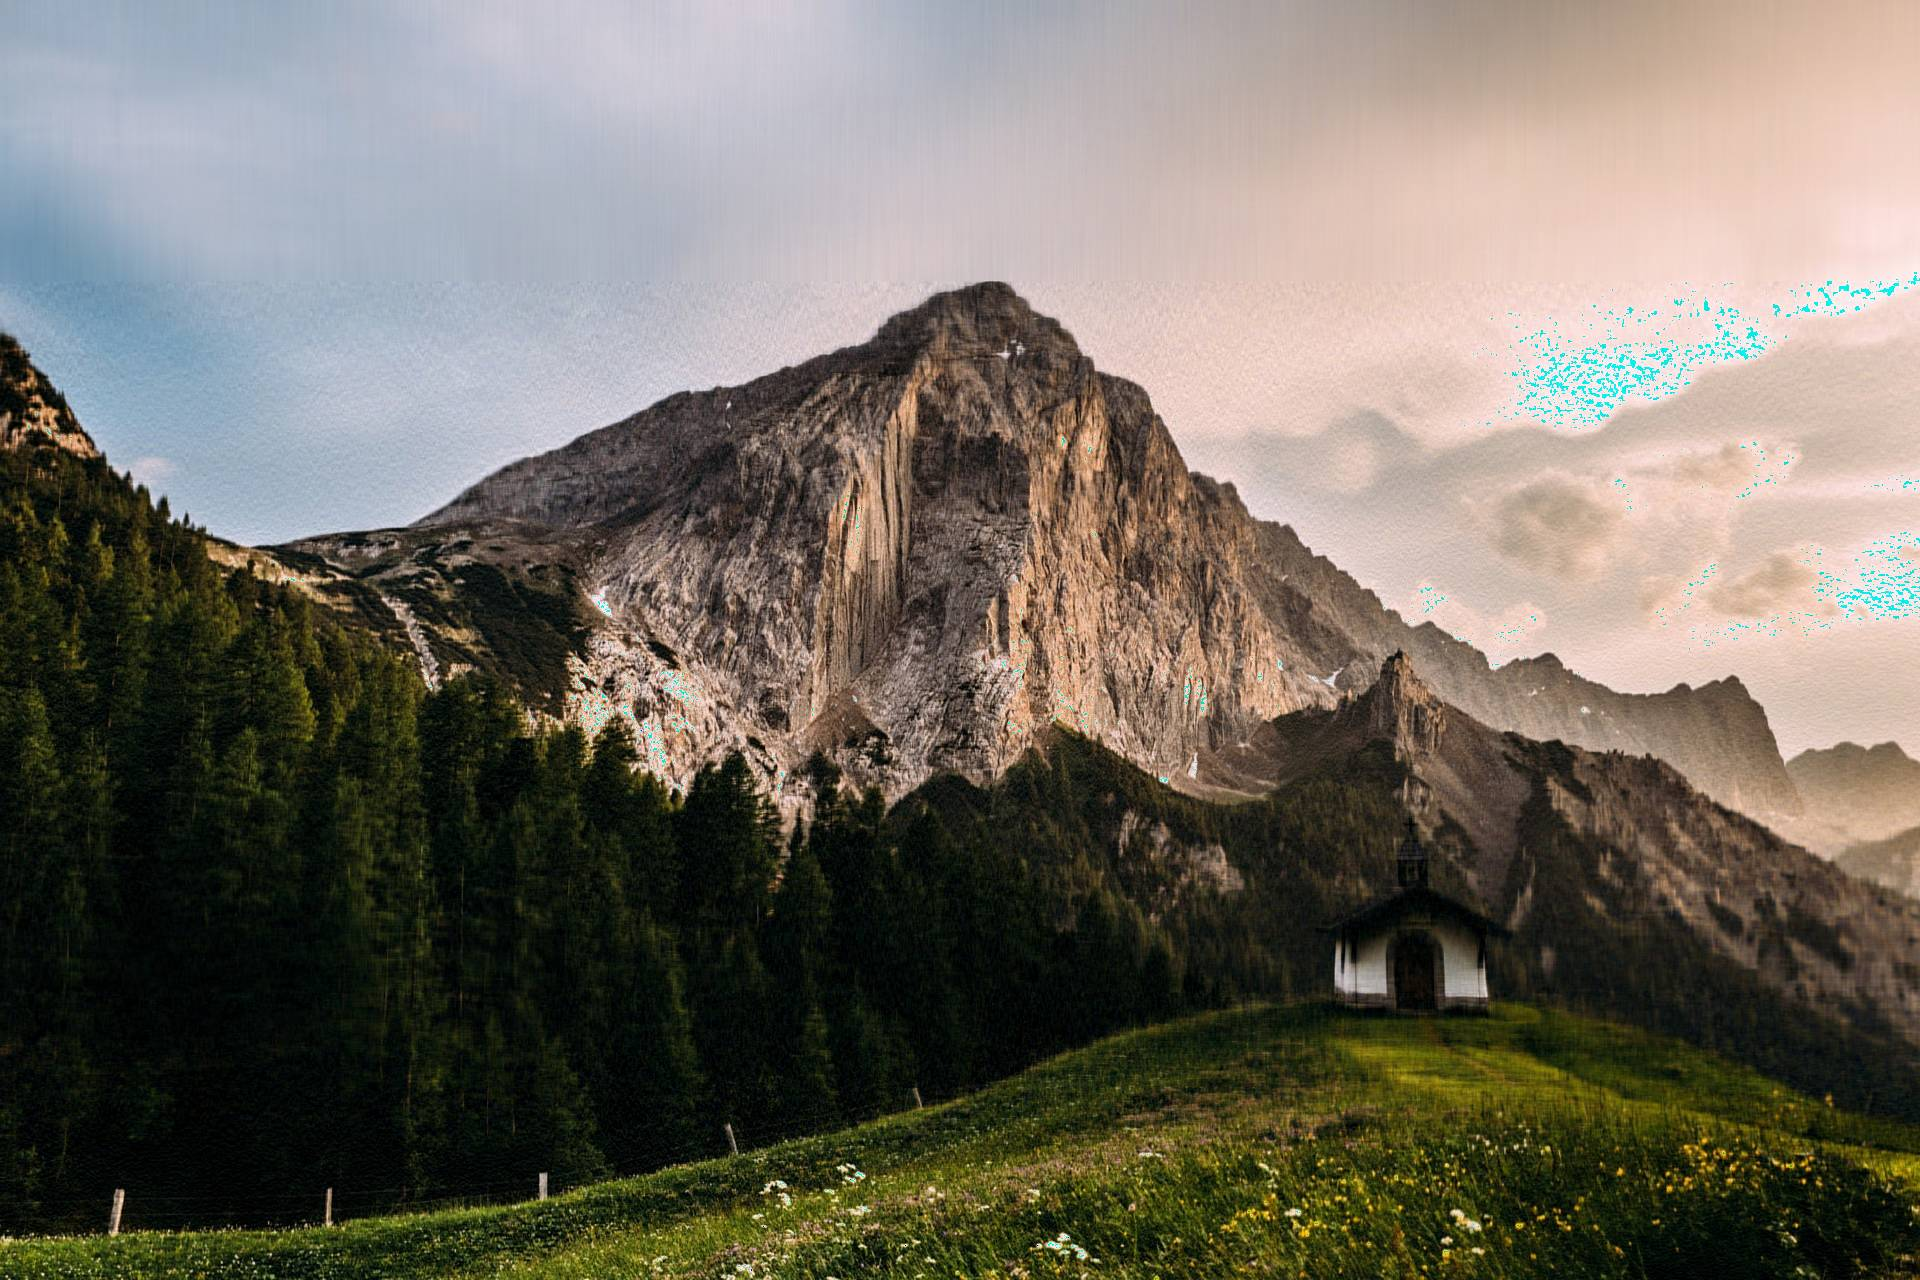
\includegraphics[width = 0.95\textwidth]{reconstructions/with_200comps_Austria.jpg}
    \label{fig:aus_200}
    \end{minipage}%
    \begin{minipage}{.45\textwidth}
      \centering
    \caption{Восстановленное изображение \\(400 компонент)}
    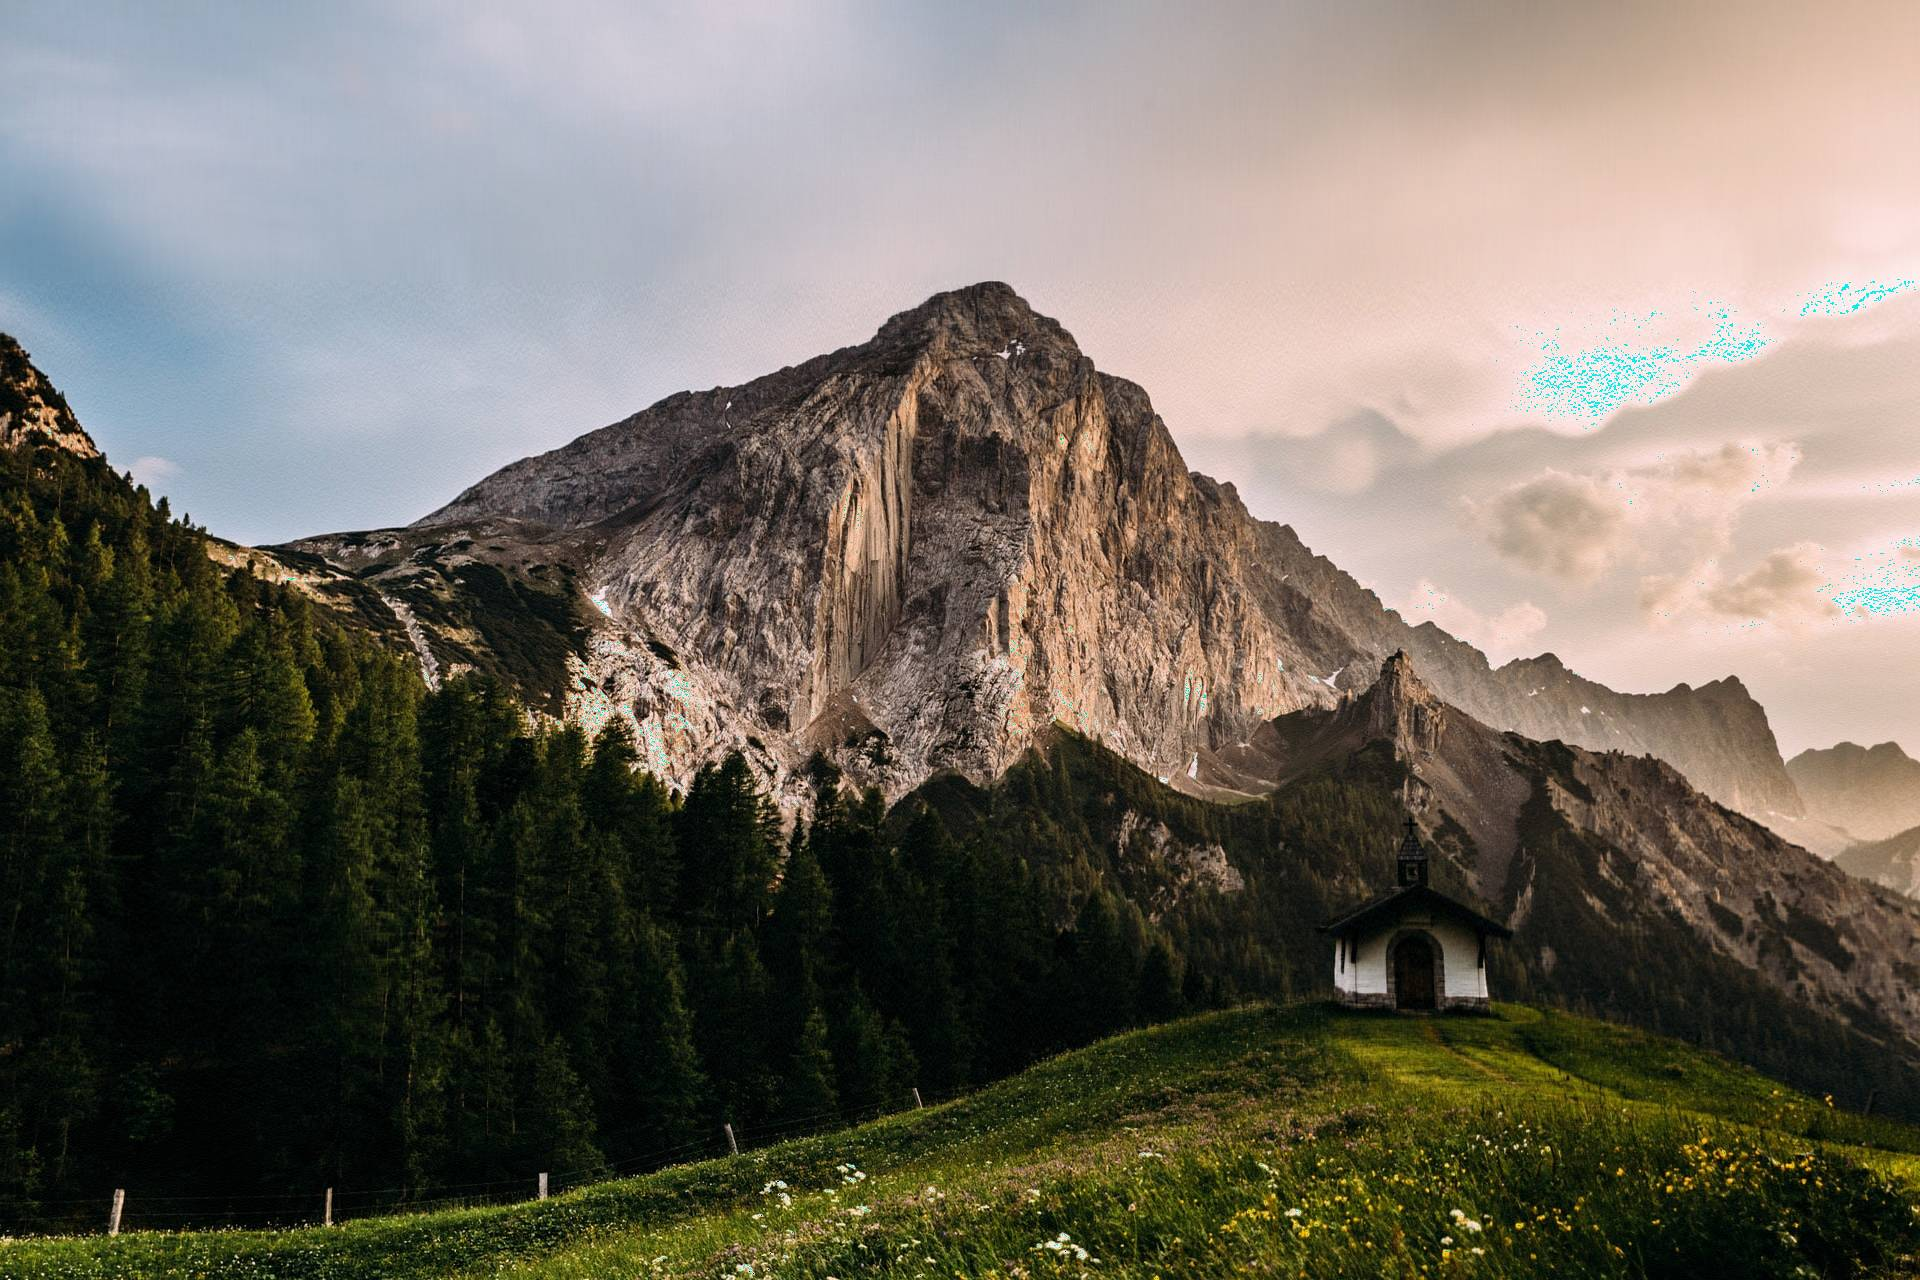
\includegraphics[width = 0.95\textwidth]{reconstructions/with_400comps_Austria.jpg}
    \label{fig:aus_400}
    \end{minipage}%
\end{figure}
\begin{table}[H]
    \centering
    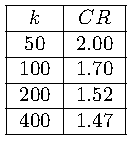
\includegraphics[]{tables/CR_for_Austria.pdf}
    \caption{Оценка сжатия первого\\цветного рисунка}
    \label{tab:aus}
\end{table}
\subsubsection{Второе изображение}
Размер оригинала - 5.09 МБ, разрешение - $5875\times 3917$ пикселя.
\begin{figure}[H]
    \centering
    \caption{Оригинал}
    \includegraphics[width = .45\textwidth]{resources/Colosseum.jpg}
    \label{fig:colos}
\end{figure}
\begin{figure}[H]
\centering
    \begin{minipage}{.45\textwidth}
    \caption{Восстановленное изображение \\(50 компонент)}
    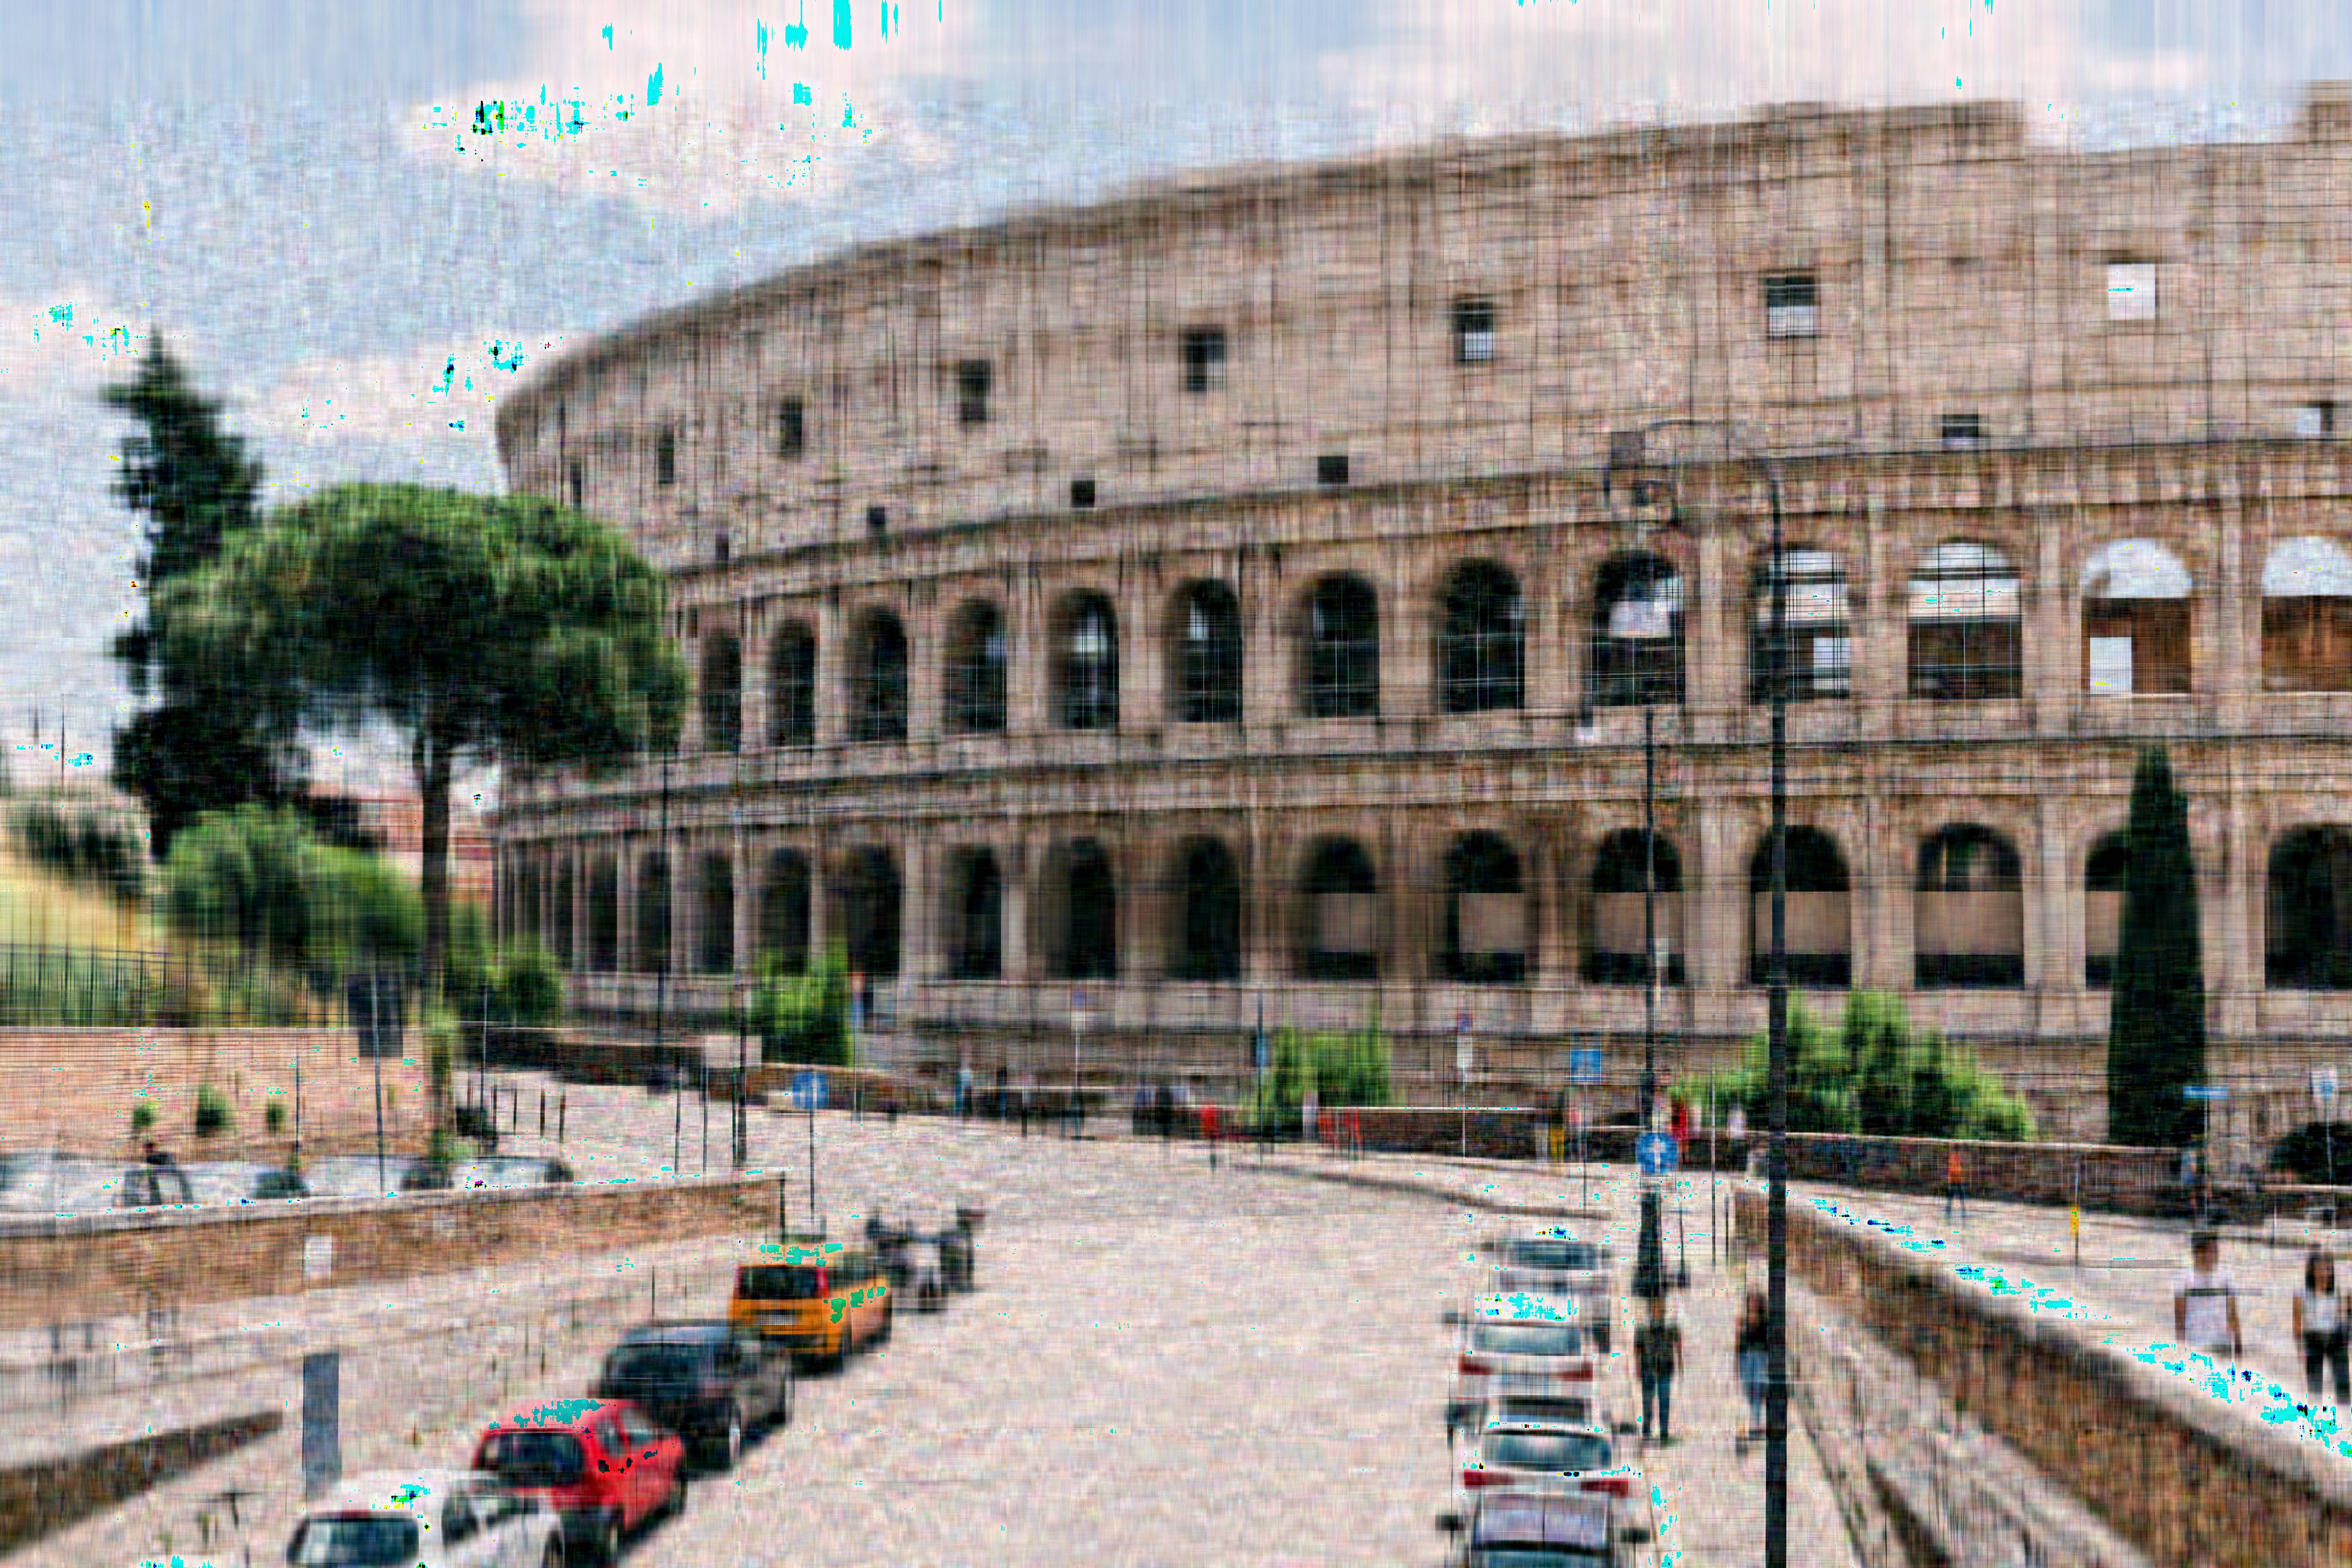
\includegraphics[width = 0.95\textwidth]{reconstructions/with_50comps_Colosseum.jpg}
    \label{fig:col_50}
    \end{minipage}%
    \begin{minipage}{.45\textwidth}
      \centering
    \caption{Восстановленное изображение \\(100 компонент)}
    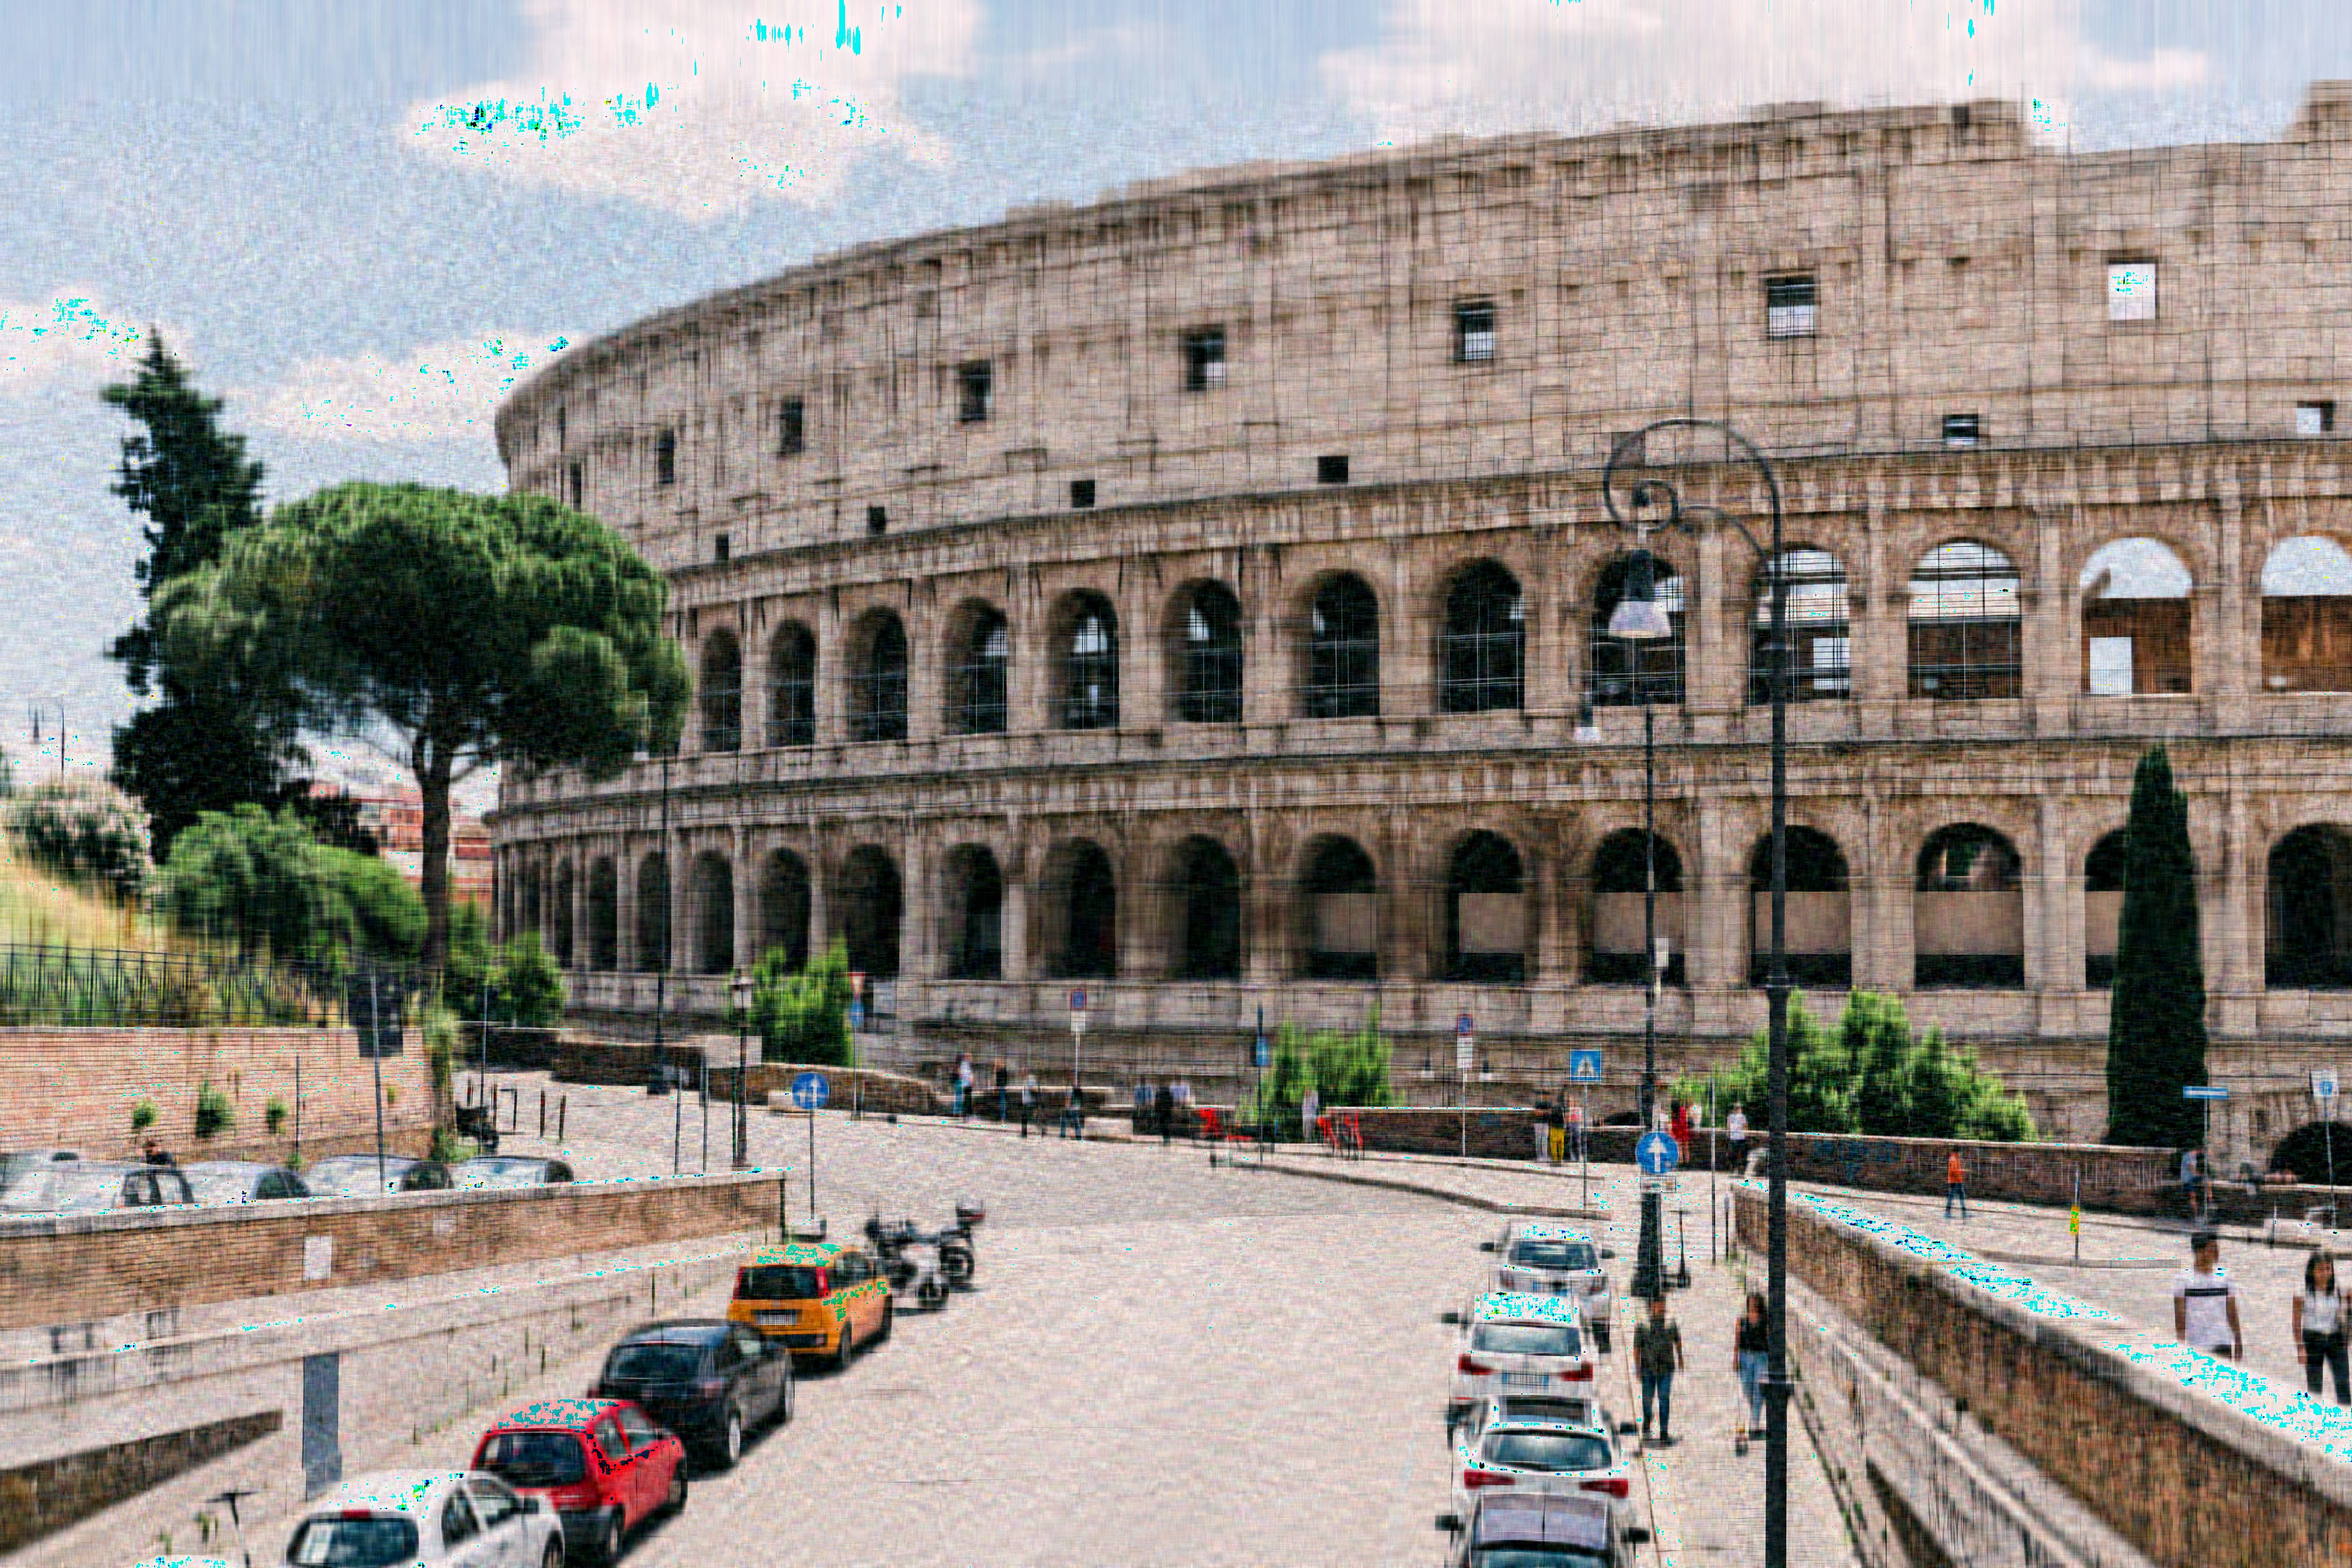
\includegraphics[width = 0.95\textwidth]{reconstructions/with_100comps_Colosseum.jpg}
    \label{fig:col_100}
    \end{minipage}%
\end{figure}
\begin{figure}[H]
\centering
    \begin{minipage}{.45\textwidth}
    \caption{Восстановленное изображение \\(200 компонент)}
    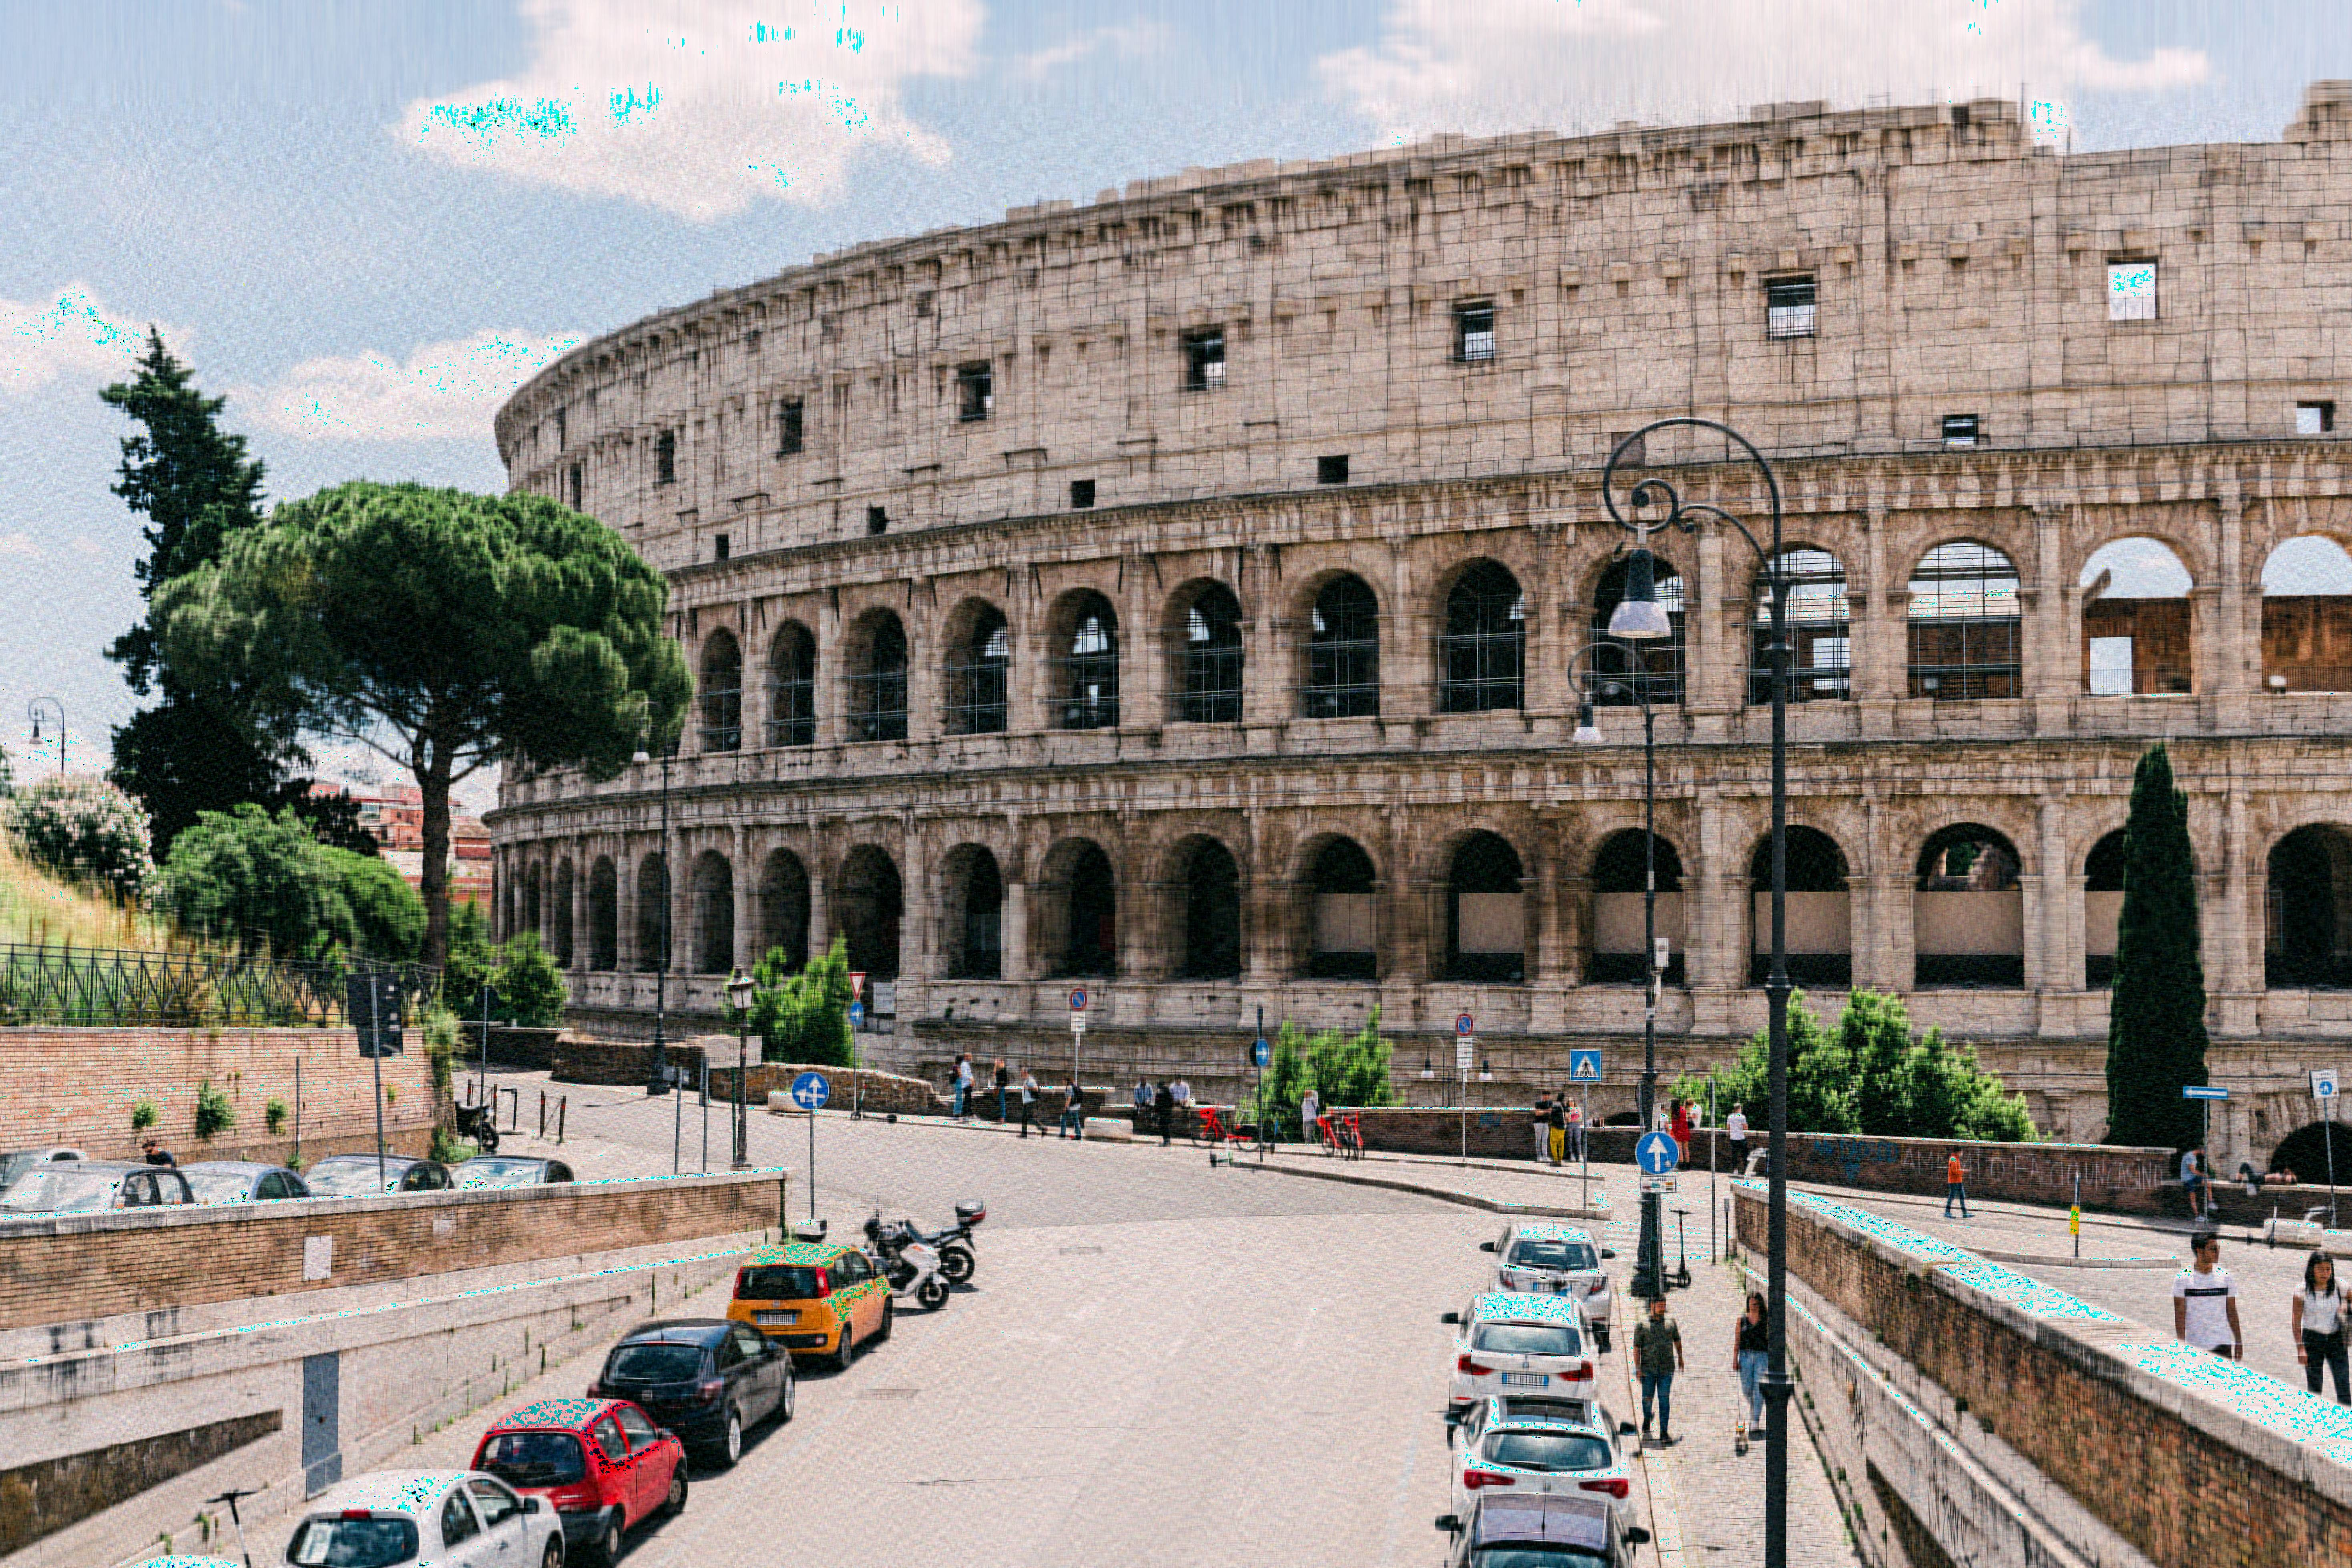
\includegraphics[width = 0.95\textwidth]{reconstructions/with_200comps_Colosseum.jpg}
    \label{fig:col_200}
    \end{minipage}%
    \begin{minipage}{.45\textwidth}
      \centering
    \caption{Восстановленное изображение \\(400 компонент)}
    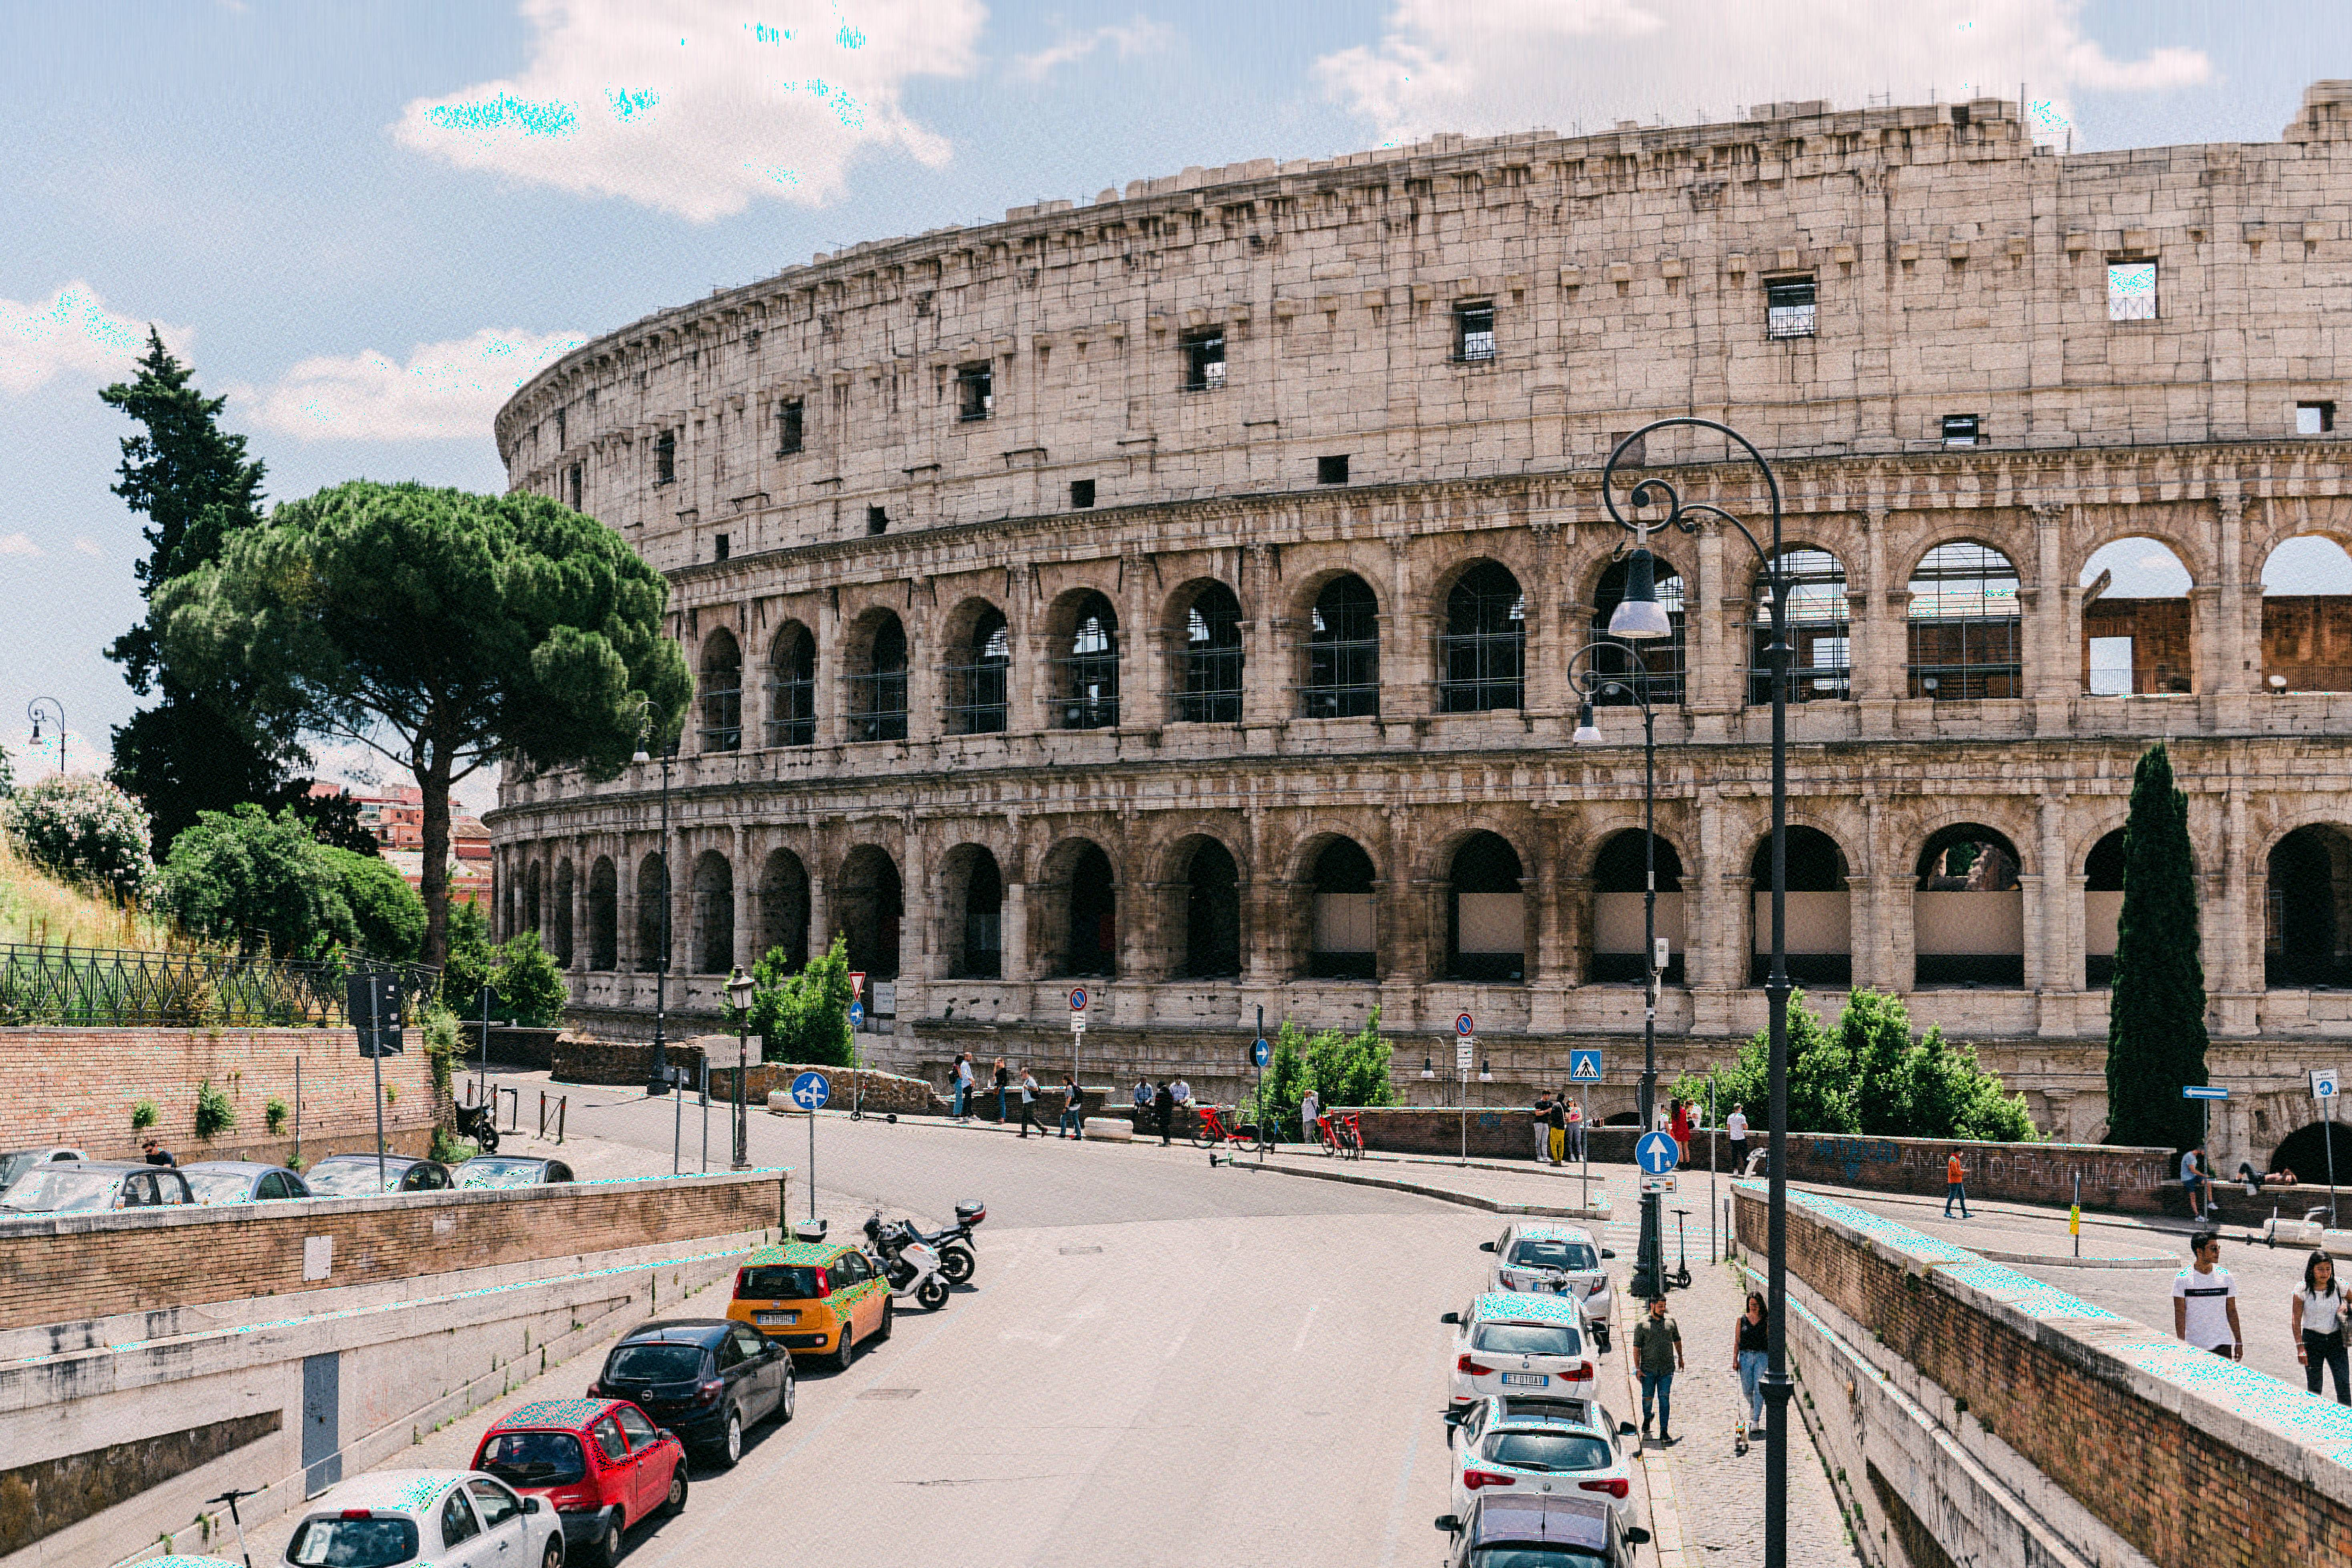
\includegraphics[width = 0.95\textwidth]{reconstructions/with_400comps_Colosseum.jpg}
    \label{fig:col_400}
    \end{minipage}%
\end{figure}
\begin{figure}[H]
\centering
    \begin{minipage}{.45\textwidth}
    \caption{Восстановленное изображение \\(800 компонент)}
    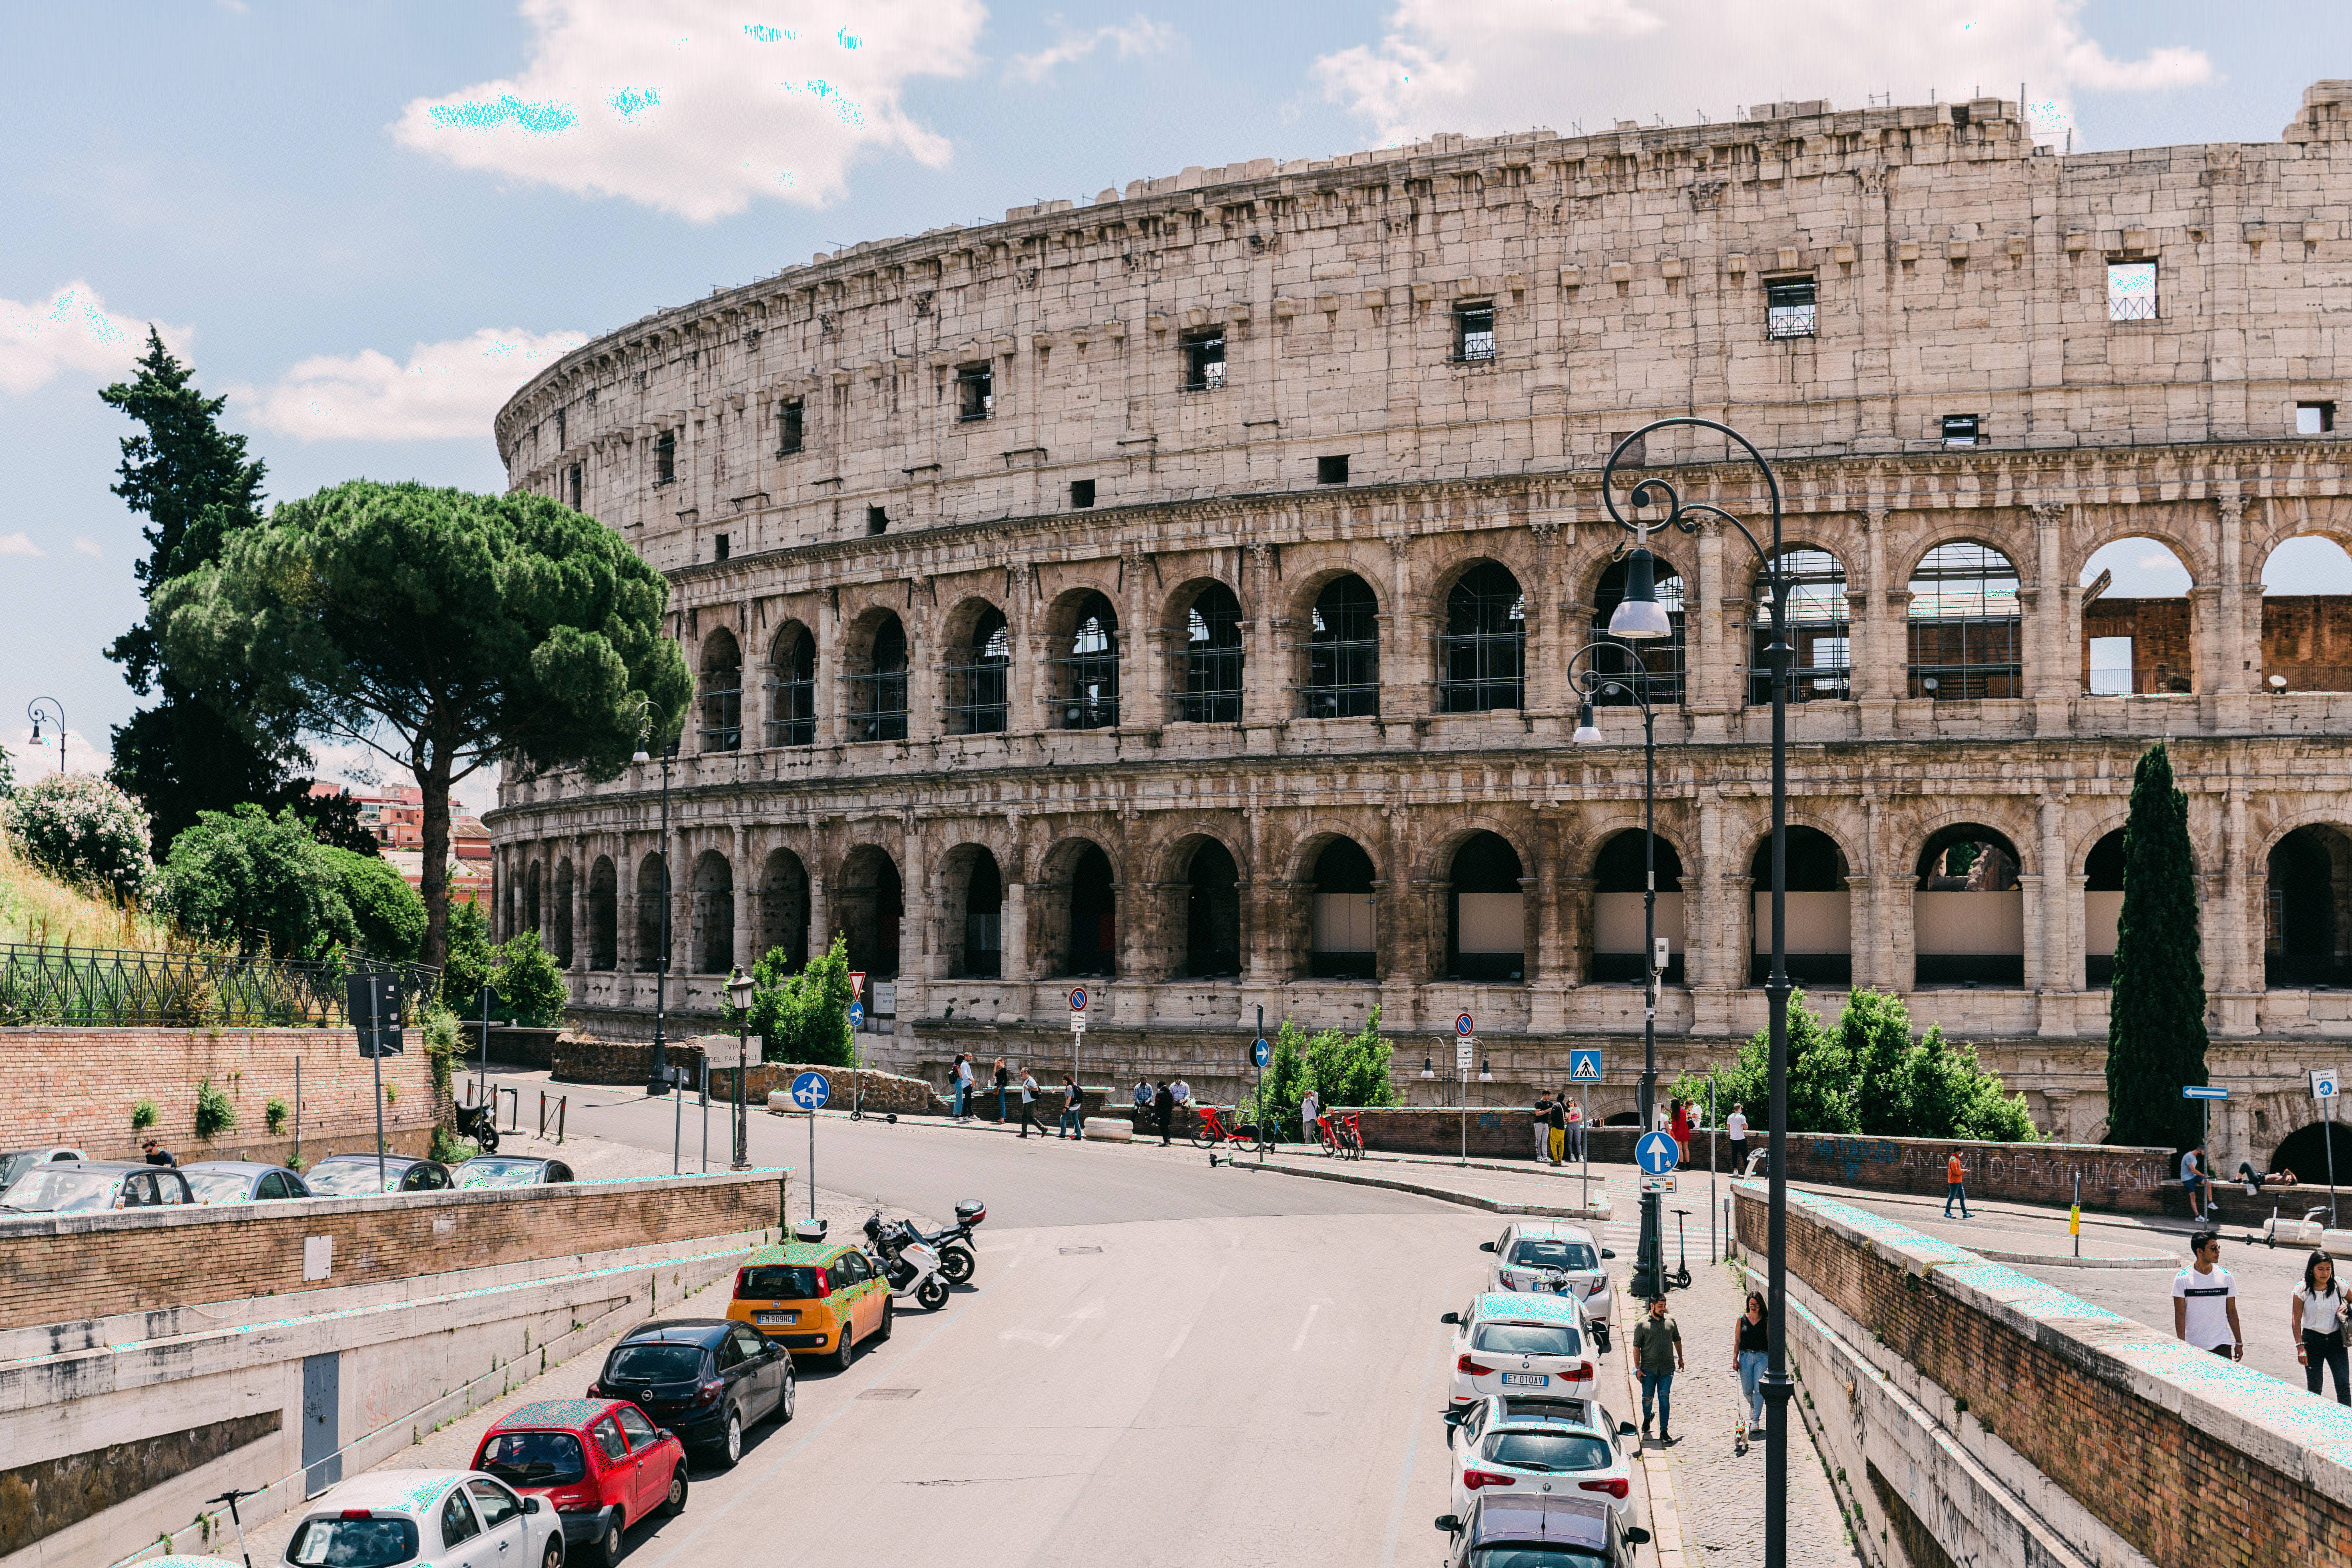
\includegraphics[width = 0.95\textwidth]{reconstructions/with_800comps_Colosseum.jpg}
    \label{fig:col_800}
    \end{minipage}%
    \begin{minipage}{.45\textwidth}
      \centering
    \caption{Восстановленное изображение \\(1200 компонент)}
    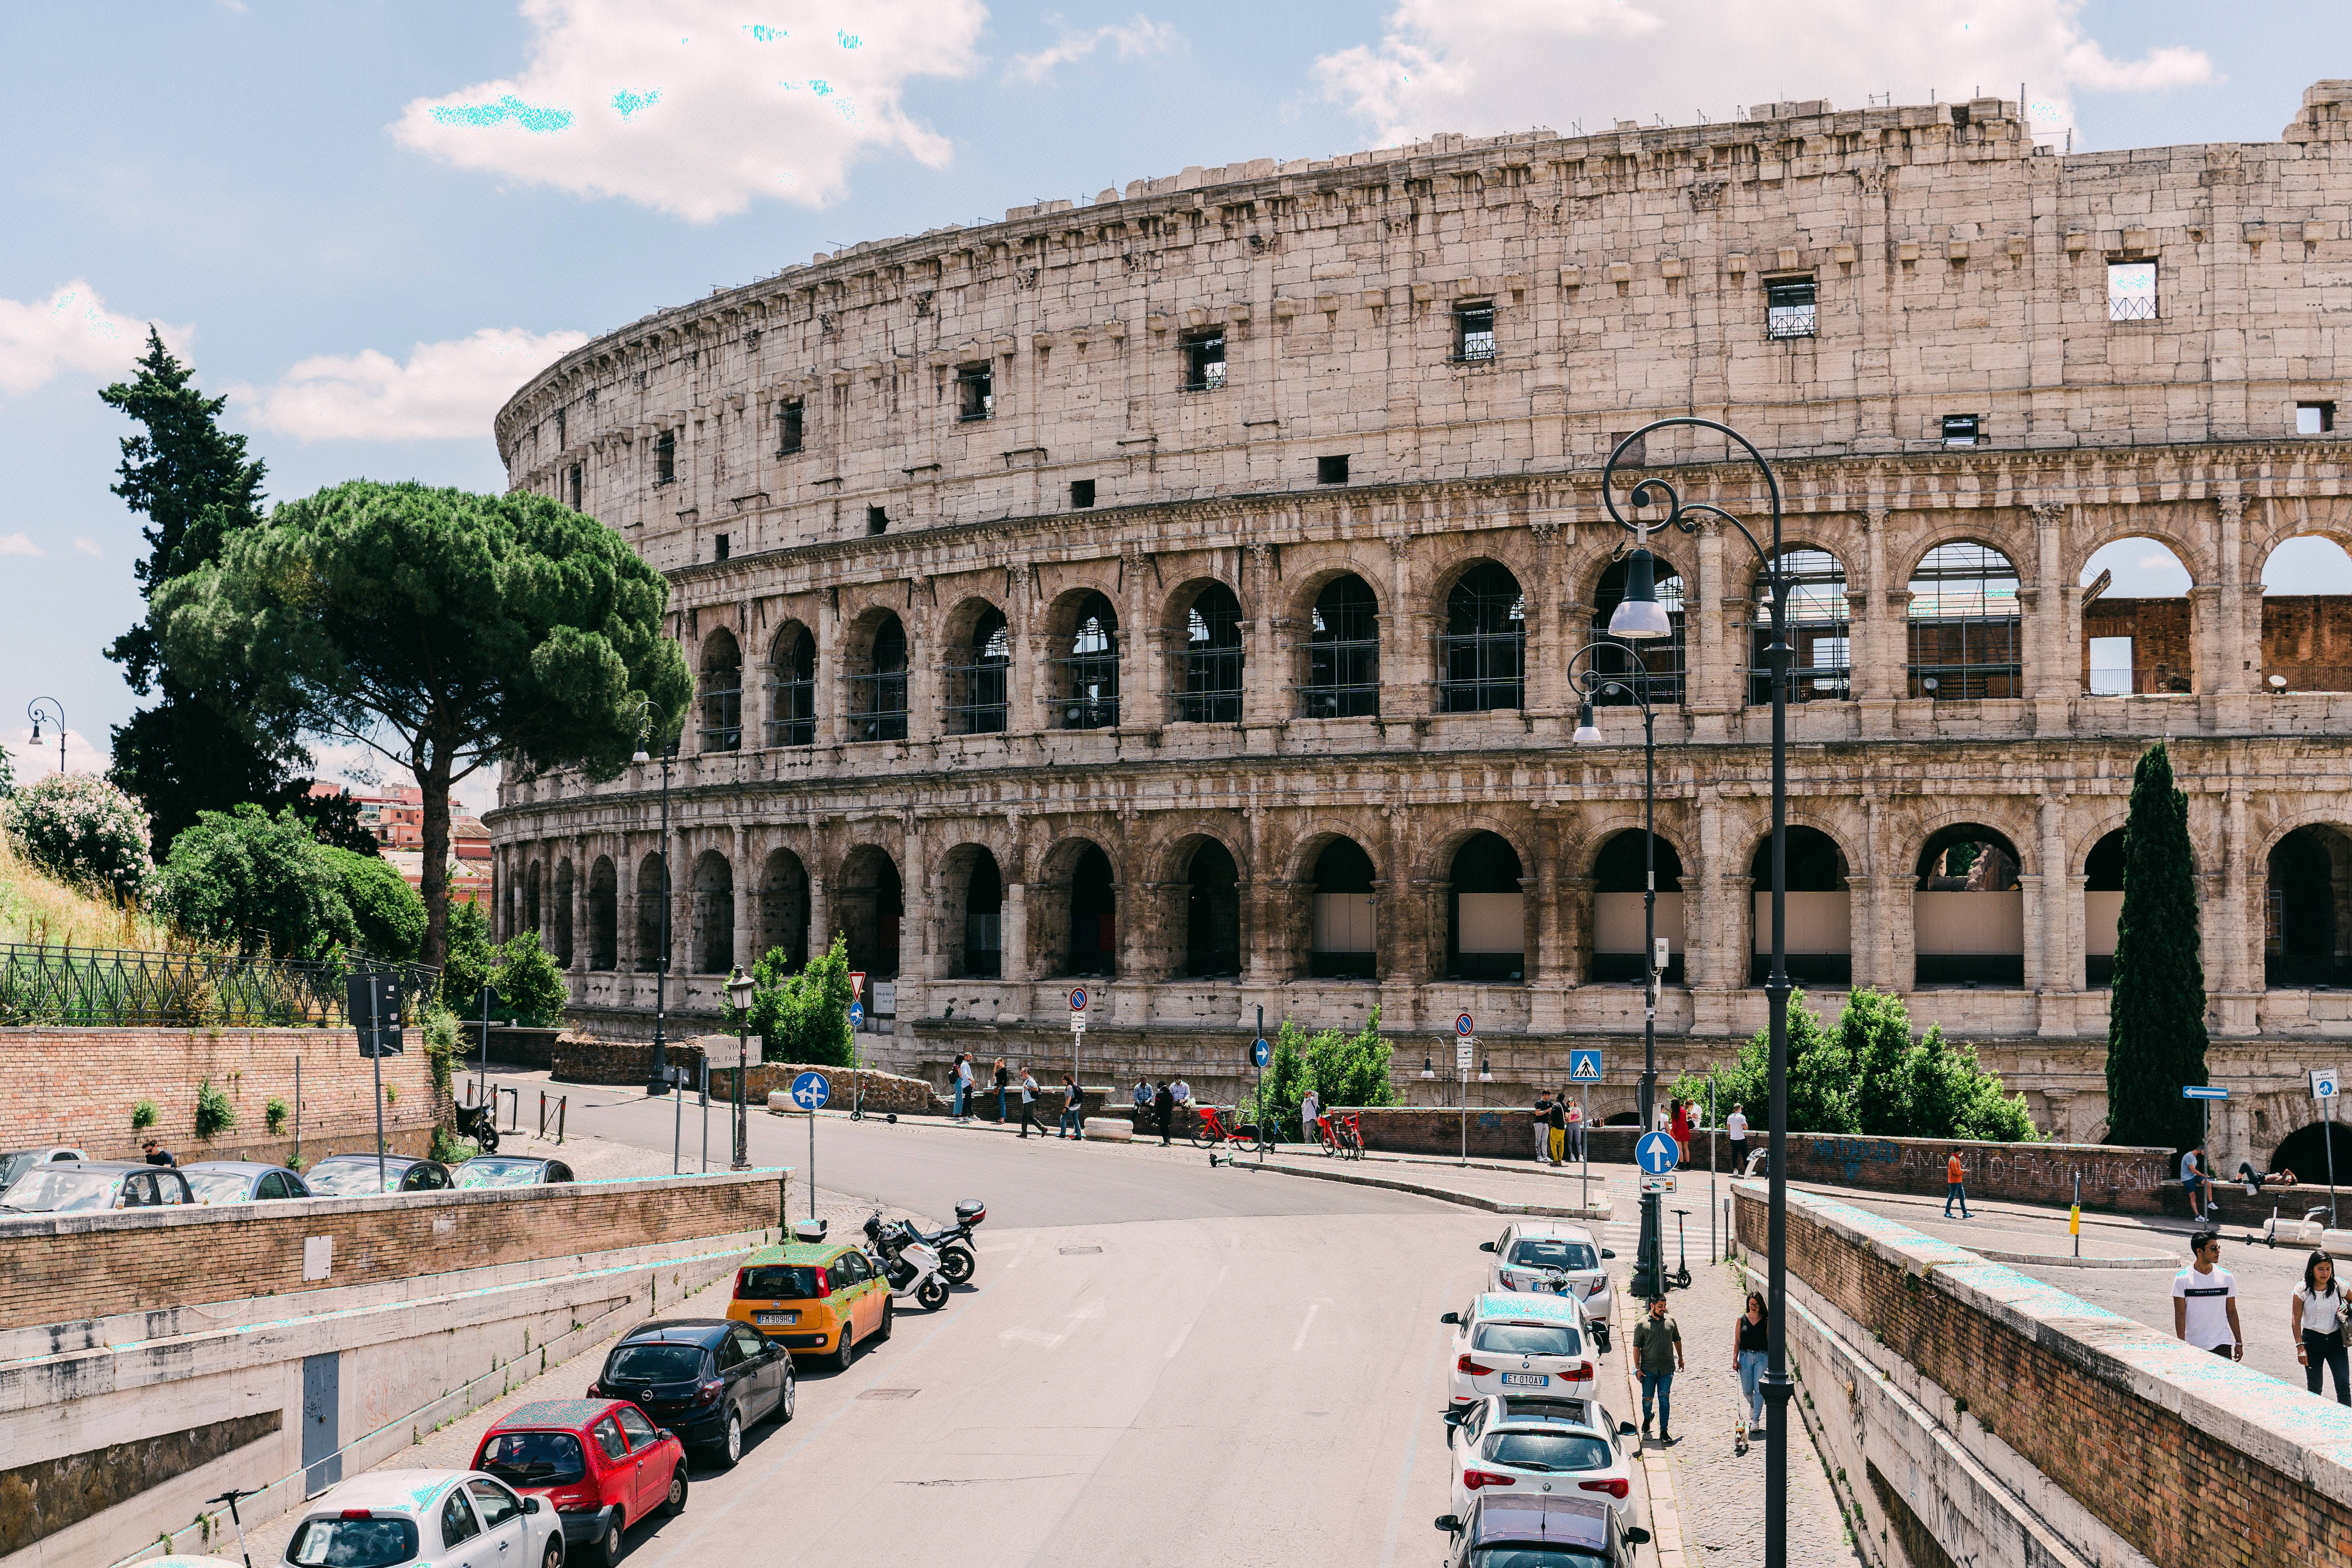
\includegraphics[width = 0.95\textwidth]{reconstructions/with_1200comps_Colosseum.jpg}
    \label{fig:col_1200}
    \end{minipage}%
\end{figure}
\begin{table}[H]
    \centering
    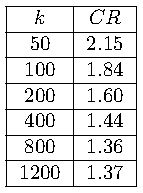
\includegraphics[]{tables/CR_for_Colosseum.pdf}
    \caption{Оценка сжатия второго\\цветного рисунка}
    \label{tab:col}
\end{table}
\section{Обсуждение}
По результатам даже данного сравнительно некрупного исследования можно сказать, что использование метода главных компонент для сжатия изображений в некоторых случаях нецелесообразно. Особенно отчетливо это видно на примере первого черно-белого рисунка: при восстановлении исходного изображения со 100 главными компонентами из 1080 изображение сжимается всего лишь в 1.24 раза, причем нельзя сказать, что результат неотличим «на глаз» от оригинала - в верхнем правом углу отчетливо наблюдается «артефакт» в виде зернистости. Эта зернистоть не пропадает и при переходе к 200 главным компонентам, при которых, однако, восстановление уже лишено смысла в силу близости степени сжатия к 1.\\
Оба цветных рисунка, если не брать во внимание небольшие синие пятна, появляющиеяся вблизи контуров облаков, «на глаз» напоминают оригинал уже при восстановлении с 400 главными компонентами. Степень сжатия для обоих рисунков в таком случае равна примерно 1.5.\\
Лучше всего метод вел себя при применении ко второму крупноразмерному черно-белому рисунку. Восстановленный при 200 главных компонентах рисунок визуально почти идентичен оригиналу и имеет степень сжатия, равную 3.26.
\section*{Примечание}
С материалами работы можно ознакомиться по ссылке: \url{https://github.com/Kozlov992/MS_TermPaper}.\\ Код работы может быть найден в файле Source.pdf, оригиналы изображений - в папке resources, восстановленные изображения - в папке reconstructions.
\begin{thebibliography}{9}
\bibitem{book1} 
J.M. isn't a mathematician (\url{shorturl.at/rtKNY}), Why is SVD on $X$ preferred to eigendecomposition of $XX^\top$ in PCA?\\URL (version: 2013-04-12): \url{https://math.stackexchange.com/q/359428}.
\bibitem{book2}
Smith, L. I. (2002, February 26). A tutorial on principal components analysis.\\
\url{http://www.cs.otago.ac.nz/cosc453/student_tutorials/principal_components.pdf}.
\bibitem{book3}
Santo Rdo E. (2012,  Apr-Jun). Principal Component Analysis applied to digital image compression.\\
\url{http://www.scielo.br/pdf/eins/v10n2/a04v10n2.pdf}.
\end{thebibliography}
\end{document}
